\documentclass[reqno,12pt]{amsart}

\usepackage[colorlinks=true]{hyperref}
\hypersetup{urlcolor=blue, citecolor=red}

\usepackage{amssymb,graphicx,color}
\usepackage[latin1]{inputenc}

\usepackage[capitalize,nameinlink,noabbrev]{cleveref}

%The Layout
\setlength{\oddsidemargin}{0pt}
\setlength{\evensidemargin}{0pt}
\setlength{\textheight}{42\baselineskip}
\setlength{\textwidth}{6in}
%\addtolength{\headheight}{0.7in}

\theoremstyle{plain} % default style for the following 
\newtheorem{theorem}{Theorem}[section]
\newtheorem{lemma}{Lemma}[section]
\newtheorem{proposition}{Proposition}[section]
\newtheorem{corollary}{Corollary}[section]
%\newtheorem{definition}{Definition}[section]
\newtheorem{problem}{Problem}[section]
\newtheorem{stdhyp}{Standing Hypothesis}[section]
\theoremstyle{definition} % definition style for the following 
\newtheorem{remark}{Remark}[section]
\newtheorem{fact}{Fact}[section]

%\newcommand{\comment}[1]{\textcolor{red}{\framebox{\parbox{0.9\textwidth}{\textbf{#1}}}}}
\newcommand{\comment}[1]{\textcolor{red}{\textbf{#1}}}
\newcommand{\doshow}[1]{#1}
\newcommand{\dontshow}[1]{}
\newcommand{\extra}[1]{\dontshow{#1}} % use \show to show the extra stuff or \donotshow not to show it

%\mathchardef\mhyphen="2D

\renewcommand{\subjclassname}{$2020$ Mathematics Subject Classification}

\renewcommand{\theenumi}{\roman{enumi}}

\begin{document}
\numberwithin{equation}{section}

% Article info

\title[Strong convergence of the Euler method for Random ODEs]{Improved error estimate for the order of strong convergence of the Euler method for random ordinary differential equations}

\author[P. E. Kloeden]{Peter E. Kloeden}
\author[R. M. S. Rosa]{Ricardo M. S. Rosa}

\address[Peter E. Kloeden]{Mathematics Department, University of Tubingen, Germany}
\address[Ricardo M. S. Rosa]{Instituto de Matem\'atica, Universidade Federal do Rio de Janeiro, Brazil}

\email[P. E. Kloeden]{kloeden@math.uni-frankfurt.de}
\email[R. M. S. Rosa]{rrosa@im.ufrj.br}

\date{\today}

\thanks{The second author was partly supported by the Laborat\'orio de Matem\'atica Aplicada, Instituto de Matem\'atica, Universidade Federal do Rio de Janeiro (LabMA/IM/UFRJ)}

\subjclass[2000]{76D05, 76D06, 35Q30, 37L99}
\keywords{random ordinary differential equations, Euler method, strong convergence, It\^o process, point process, fractional Brownian motion}.

\begin{abstract}
It is well known that the Euler method for approximating the solutions of a random ordinary differential equation $\mathrm{d}X_t/\mathrm{d}t = f(t, X_t, Y_t)$ driven by a stochastic process $\{Y_t\}_t$ with $\theta$-H\"older sample paths is estimated to be of strong order $\theta$ with respect to the time step, provided $f=f(t, x, y)$ is sufficiently regular and with suitable bounds. Here, it is proved that, in many typical cases, further conditions on the noise can be exploited so that the strong convergence is actually of order 1, regardless of the H\"older regularity of the sample paths. This applies for instance to additive or multiplicative It\^o  process noises (such as Wiener, Ornstein-Uhlenbeck, and Geometric Brownian motion process); to point-process noises (such as Poisson point processes and Hawkes self-exciting processes, which even have jump-type discontinuities); and to transport-type processes with sample paths of bounded variation. The result is based on a novel approach, estimating the global error as an iterated integral over both large and small mesh scales, and switching the order of integration to move the critical regularity to the large scale. The work is complemented with numerical simulations illustrating the strong order 1 convergence in those cases, and with an example with fractional Brownian motion noise with Hurst parameter $0 < H < 1/2$ for which the order of convergence is $H + 1/2$, hence lower than the attained order 1 in the examples above, but still higher than the order $H$ of convergence expected from previous works.
\end{abstract}

\maketitle

\section{Introduction}

Consider the following initial value problem for a \textbf{random ordinary differential equation (RODE)}:
\begin{equation}
  \label{rodeeq}
  \begin{cases}
    \displaystyle \frac{\mathrm{d}X_t}{\mathrm{d} t} = f(t, X_t, Y_t), & 0 \leq t \leq T, \\
    \left. X_t \right|_{t = 0} = X_0,
  \end{cases}
\end{equation}
on a time interval $I=[0, T]$, with $T > 0$, and where the noise $\{Y_t\}_{t\in I}$ is a given stochastic process. This can be a scalar or a system of equations and the noise can also be either scalar or vector valued. The sample space is denoted by $\Omega$.

The Euler method for solving this initial value problem consists in approximating the solution on a uniform time mesh $t_j = j\Delta t_N$, $j = 0, \ldots, N$, with fixed time step $\Delta t_N = T/N$, for a given $N\in \mathbb{N}$. In such a mesh, the Euler scheme takes the form
\begin{equation}
  \label{emscheme}
  \begin{cases}
    X_{t_j}^N = X_{t_{j-1}}^N + \Delta t_N f(t_{j-1}, X_{t_{j-1}}^N, Y_{t_{j-1}}), & j = 1, \ldots, N, \\
    X_0^N = X_0.
  \end{cases}
\end{equation}
Notice $t_j = j\Delta t_N = jT/N$ also depends on $N$, but we do not make this dependency explicit, for the sake of notational simplicity.

We are interested in the order of \emph{strong} convergence, i.e. convergence in square mean: the approximation $\{X_{t_j}^N\}_j$ is said to converge to $\{X_t\}_t$ with strong order $\theta>0$ when there exists a constant $C \geq 0$ such that
\begin{equation}
    \label{strongordertheta}
    \max_{j=0, \ldots, N}\mathbb{E}\left[ \left\| X_{t_j} - X_{t_j}^N \right\| \right] \leq C \Delta t_N^\theta, \qquad \forall N \in \mathbb{N},
\end{equation}
where $\mathbb{E}[\cdot]$ indicates the expectation of a random variable on $\Omega$, and $\|\cdot\|$ is the norm in the appropriate space. There are other important notions of convergence, such as weak convergence, $p$-th mean convergence, and pathwise convergence (see e.g. \cite{HanKloeden2017,HighamKloeden2021, JentzenKloeden2011}), but we focus on strong convergence, here.

Under certain regularity conditions on $f$, it is proved in \cite{GruneKloeden2001} that, when the noise $\{Y_t\}_{t\in I}$ has $\theta$-H\"older continuous sample paths, the Euler scheme converges to the exact solution in the \emph{pathwise} sense with order $\theta$ with respect to the time step. Under global uniformity conditions on the nonlinear term, the same approach in \cite{GruneKloeden2001} also yields the convergence of order $\theta$ in the \emph{strong} sense \eqref{strongordertheta}.

Our aim is to show that, in many classical examples, it is possible to exploit further conditions that yield in fact a higher \emph{strong} order of convergence, with the sample noise paths still being H\"older continuous or even discontinuous. This is the case, for instance, when the noise is a point process, a transport process, or an It\^o process, for which the convergence is of strong order 1. It is also the case for fractional Brownian motion noise with Hurst parameter $H$, for which the sample paths are $H$-H\"older continuous, but the strong convergence is of order 1, when $1/2 \leq H < 1$, and of order $H + 1/2$, when $0 < H < 1/2$, which is still higher than the H\"older exponent $H$ of the sample paths.

The global conditions on the nonlinear term are natural assumption when looking for strong convergence. Pathwise convergence, on the other hand, usually requires less stringent conditions (see e.g. \cite{JentzenKloedenNeuenkirch2009, JentzenKloeden2011}), but those are not the subject of interest here. The possibility of extending the improved order of strong convergence to pathwise convergence seems feasible for the case of sample paths of bounded variation but not so much for It\^o process noises for which the It\^o isometry is of fundamental importance. These will be investigated in a future oportunity.

The first main idea of the proof is to not estimate the local error and, instead, work with an explicit formula for the global error (see \cref{lemglobalerrorintegralformula}), namely
\begin{equation}
    \label{lemglobalerrorintegralformulaintro}
    \begin{aligned}
        X_{t_j} - X_{t_j}^N & = X_0 - X_0^N + \int_0^{t_j} \left( f(s, X_s, Y_s) - f(s, X_{\tau^N(s)}, Y_s) \right)\;\mathrm{d}s  \\ 
        & \qquad + \int_{0}^{t_j} \left( f(s, X_{\tau^N(s)}, Y_s) - f(s, X_{\tau^N(s)}^N, Y_s) \right)\;\mathrm{d}s \\
        & \qquad + \int_0^{t_j} \left( f(s, X_{\tau^N(s)}^N, Y_s) - f(\tau^N(s), X_{\tau^N(s)}^N, Y_{\tau^N(s)}) \right)\;\mathrm{d}s,
    \end{aligned}
\end{equation}
for $j = 1, \ldots, N,$ where $\tau^N$ is a piecewise constant function with jumps at the mesh points $t_j$ (see \eqref{tauNt}).

The first term vanishes due to the initial condition $X_0^N = X_0$. The second term only depends on the solution and can be easily estimated with natural regularity conditions on the term $f=f(t, x, y)$. The third term is handled solely with the typical required condition on $f=f(t, x, y)$ of being uniformly globally Lipschitz continuity with respect to $x$. With those, we obtain the following basic bound for the global error (see \cref{lembasicestimate})
\begin{multline}
    \label{Etjbasicboundintro}
        \|X_{t_j} - X_{t_j}^N\| \leq \left( \|X_0 - X_0^N\| + L_X \int_0^{t_j} \|X_s - X_{\tau^N(s)}\| \;\mathrm{d}s \right. \\
        \left. \left\|\int_0^{t_j} \left( f(s, X_{\tau^N(s)}^N, Y_s) - f(\tau^N(s), X_{\tau^N(s)}^N, Y_{\tau^N(s)}) \right)\;\mathrm{d}s\right\|\right) e^{L_X t_j}.
\end{multline}

The only problematic, noise-sensitive term is the last one. The classical analysis is to use an assumed $\theta$-H\"older regularity of the noise sample paths and estimate the local error as
\[
    \mathbb{E}\left[\left\|f(s, X_{\tau^N(s)}^N, Y_s) - f(\tau^N(s), X_{\tau^N(s)}^N, Y_{\tau^N(s)})\right\|\right] \leq C\Delta t_N^{\theta}.
\]
Instead, we look at the whole noise error 
\[
    \mathbb{E}\left[\left\|\int_0^{t_j} \left( f(s, X_{\tau^N(s)}^N, Y_s) - f(\tau^N(s), X_{\tau^N(s)}^N, Y_{\tau^N(s)}) \right)\;\mathrm{d}s\right\|\right]
\]
and assume that the steps of the process given by $F_t = f(t, X_{\tau^N(t)}^N, Y_t)$ can be controlled in a suitable global way. In order to give the main idea, let us consider a scalar equation with a scalar noise and assume that the sample paths of $\{F_t\}_{t\in I}$ satisfy
\[
    F_s - F_\tau = \int_\tau^s \;\mathrm{d}F_\xi,
\]
either in the sense of a Riemann-Stieltjes integral or of an It\^o integral. The first sense fits the case of noises with bounded total variation, while the second one fits the case of an It\^o process noise. In any case, we bound the global error term using the Fubini Theorem,
\begin{multline*}
    \int_0^{t_j} \left( f(s, X_{\tau^N(s)}^N, Y_s) - f(\tau^N(s), X_{\tau^N(s)}^N, Y_{\tau^N(s)}) \right)\;\mathrm{d}s = \int_0^{t_j} \int_{\tau^N(s)}^s \;\mathrm{d}  F_\xi\;\mathrm{d}s \\
    = \int_0^{t_j} \int_{\xi}^{\tau^N(\xi) + \Delta t_N} \;\mathrm{d}s \;\mathrm{d} F_\xi  = \int_0^{t_j} (\tau^N(\xi) + \Delta t_N - \xi) \;\mathrm{d} F_\xi.
\end{multline*}
Then, we find that
\begin{multline*}
    \mathbb{E}\left[\left\| \int_0^{t_j} \left( f(s, X_{\tau^N(s)}^N, Y_s) - f(\tau^N(s), X_{\tau^N(s)}^N, Y_{\tau^N(s)}) \right)\;\mathrm{d}s\right\|\right] \\
    \leq \mathbb{E}\left[\left\| \int_0^{t_j} (\tau^N(\xi) + \Delta t_N - \xi) \;\mathrm{d} F_\xi \right\|\right].
\end{multline*}

In the case of an It\^o process noise, we assume
\[
    \mathrm{d}F_t = A_t\;\mathrm{d}t + B_t\;\mathrm{d}W_t,
\]
with adapted processes $\{A_t\}_t$, $\{B_t\}_t$, which may actually depend on $\{Y_t\}_t$, so that multiplicative noise is allowed. Then, in this case, we bound the right hand side using the Lyapunov inequality and the It\^o isometry:
\begin{multline*}
    \mathbb{E}\left[\left\| \int_0^{t_j} (\tau^N(\xi) + \Delta t_N - \xi) \;\mathrm{d} F_\xi \right\|\right] \\
    \leq \int_0^{t_j} (\tau^N(\xi) + \Delta t_N - \xi) \mathbb{E}[\|A_\xi\|] \;\mathrm{d}\xi + \left( \int_0^{t_j} (\tau^N(\xi) + \Delta t_N - \xi)^2 \mathbb{E}[\|B_\xi\|^2]\;\mathrm{d} \xi\right)^{1/2} \\ 
    \leq \Delta t_N\left(\int_0^{t_j} \mathbb{E}[\|A_\xi\|]\;\mathrm{d} \xi + \left( \int_0^{t_j} \mathbb{E}[\|B_\xi\|^2] \;\mathrm{d}\xi \right)^{1/2} \right).
\end{multline*}
which yields the strong order 1 convergence, provided the integrals are finite.

In the case of noises with bounded variation, we may actually relax the above condition and assume the steps are bounded by a process $\{\bar F_t\}_{t\in I}$ with monotonic non-decreasing sample paths,
\[
    \left\|f(s, X_{\tau^N(s)}^N, Y_s) - f(\tau^N(s), X_{\tau^N(s)}^N, Y_{\tau^N(s)})\right\| \leq \bar F_s - \bar F_{\tau^N(s)}.
\]
Using the monotonicity, this implies
\[
    \mathbb{E}\left[\left\| \int_0^{t_j} (\tau^N(\xi) + \Delta t_N - \xi) \;\mathrm{d} \bar F_\xi \right\|\right] \leq \Delta t_N \left(\mathbb{E}[\bar F_{t_j}] - \mathbb{E}[\bar F_0]\right),
\]
yielding, again, strong order 1 convergence.

These two cases are treated in \cref{secmonotonicbound} and \cref{secItonoise}. The case of bounded variation is treated in \cref{secmonotonicbound}, while the It\^o process noise case is treated in \cref{secItonoise}.

The core results in these sections are \cref{lemmonotonicbound} and \cref{thmmonotonicbound}, for the bounded variation case, and \cref{lemItostep} and \cref{thmItostep}, for the It\^o process noise case. The conditions in such results, however, are not readily verifiable. With that in mind, \cref{thmdiffmonotonicbound} and \cref{thmItonoise} give more explicit conditions for each of these two cases. Essentially, $f=f(t, x, y)$ is required to have minimal regularity in the sense of differentiability and growth conditions, while the noise $\{Y_t\}_{t\in I}$ is either required to have sample paths of bounded variation or to be an It\^o process noise.

These two types of noises can also appear at same time, in a given equation or system of equations, as treated in \cref{secmixed}. This can be regarded as a vector-valued noise, where the components of the noise may either be of bounded variation or of It\^o type. See \cref{thmmixedcase} and \cref{thmmixedcasepractical}.

We complement this work with a couple of explicit examples and their numerical implementation, illustrating the strong order 1 convergence in the cases above. We start with a system of linear equations with all sorts of noises, emcompassing noises with sample paths with bounded variation and It\^o process noises. We also implement a nonlinear toogle-switch model of gene expression driven by a combination of a compound Poisson process and a geometric Brownian motion process, illustrating, again, the two main types of noises considered here, namely a point-process with bounded variation and a multiplicative It\^o process noise.

We also include an example with a fractional Brownian motion noise (fBm), for which the order of convergence drops to $H + 1/2$, when the Hurst parameter is in the range $0 < H < 1/2$. We do not have a general proof of this order of convergence in the case of fBm noise, but we prove it here in a particular linear equation. In this example, we essentially have (see \eqref{stepfBm} and \eqref{BHtintegralformulastep})
\[
    F_s - F_\tau \sim \int_\tau^s (s-\tau)^{H-1/2}\;\mathrm{d}W_\xi + \text{higher order term}.
\]
In this case, disregarding the higher order term,
\begin{align*}
    \int_0^{t_j} & \left( f(s, X_{\tau^N(s)}^N, Y_s) - f(\tau^N(s), X_{\tau^N(s)}^N, Y_{\tau^N(s)}) \right)\;\mathrm{d}s \\ 
    & \qquad \sim \int_0^{t_j} \int_{\tau^N(s)}^s (s-\tau^N(s))^{H-1/2} \;\mathrm{d} W_\xi\;\mathrm{d}s \\
    & \qquad = \int_0^{t_j} \int_{\xi}^{\tau^N(\xi) + \Delta t_N} (s-\tau^N(s))^{H-1/2} \;\mathrm{d}s \;\mathrm{d} W_\xi \\
    & \qquad \sim \int_0^{t_j} (\tau^N(\xi) + \Delta t_N - \tau^N(\xi))^{H+1/2} \;\mathrm{d} W_\xi \\
    & \qquad = (\Delta t_N)^{H+1/2} \int_0^{t_j} \;\mathrm{d} W_\xi.
\end{align*}
which, upon taking the expectation of the absolute value, yields a strong convergence of order $H + 1/2$.

Further examples can be found in the github repository \cite{RODEConvEM2023}, such as a logistic model of population dynamics with random coefficients, loosely inspired by \cite[Section 15.2]{HanKloeden2017}, with an extra random term representing harvest; a toggle-switch model of gene expression similar to \cite[Section 7.8 ]{Asai2016}, originated from \cite{VerdCrombachJaeger2014}, see also \cite{StrasserTheisMarr2012}, driven by a combination of a compound Poisson process and a geometric Brownian motion process, illustrating, again, the two main types of noises considered here, namely a point-process with bounded variation and a multiplicative It\^o process noise; a mechanical structure model driven by a random disturbance simulating seismic ground-motion excitations in the form of a transport process, inspired by the Bogdanoff-Goldberg-Bernard model in \cite{BogdanoffGoldbergBernard1961} (see also \cite[Chapter 18]{NeckelRupp2013}, \cite{HousnerJenning1964}, and \cite{Kanai1957}, with this and other models, such as the  ubiquotous Kanai-Tajimi and Clough-Penzien colored-noise models); and a Fisher-KPP partial differential equation with random boundary conditions, as inspired by the works of \cite{SalakoShen2020} and \cite{FreidlinWentzell1992} (see also \cite{Fisher1937} and \cite{KPP1937}).

\section{Pathwise solutions}
\label{secpathwisesolution}

For the notion and main results on pathwise solution for RODEs, we refer the reader to \cite[Section 2.1]{HanKloeden2017} and \cite[Section 3.3]{NeckelRupp2013}.

We start with a fundamental set of conditions that imply the existence and uniqueness of pathwise solutions of the RODE \eqref{rodeeq} in the sense of Carath\'eodory:

\begin{stdhyp}
    \label{standinghypotheses1}
    We consider a function $f=f(t, x, y)$ defined on $I\times \mathbb{R}^d\times\mathbb{R}^k$ and with values in $\mathbb{R}^d$, and an $\mathbb{R}^k$-valued stochastic process $\{Y_t\}_{t\in I}$, where $I=[0, T]$, $T > 0$, and $d, k\in \mathbb{N}.$ We make the following standing assumptions:
    \begin{enumerate}
        \item \label{standinghypotheses1Lx} $f$ is globally Lipschitz continuous on $x$, uniformly in $t$ and $y$, i.e. there exists a constant $L_X \geq 0$ such that
            \begin{equation}
                \label{Lxassumptionbasic}
                \|f(t, x_1, y) - f(t, x_2, y)\| \leq L_X \|x_1 - x_2\|, \quad \forall t \in I, \;\forall x_1, x_2, y\in\mathbb{R}^k.
            \end{equation}

        \item \label{standinghypotheses1Car} The mapping $(t, x) \mapsto f(t, x, Y_t)$ satisfies the Carath\'eodory conditions:
            \begin{enumerate}
                \item The mapping $x \mapsto f(t, x, Y_t(\omega))$ is continuous in $\mathbb{R}^d$, for almost every $(t, \omega)\in I\times \Omega$;
                \item The mapping $t \mapsto f(t, x, Y_t(\omega))$ is Lebesgue measurable in $t\in I$, for each $x\in \mathbb{R}^d$ and each sample path $t \mapsto Y_t(\omega)$;
                \item \label{standinghypotheses1Carboundonf} The bound $\|f(t, x, Y_t)\| \leq M_t + L_X\|x\|$ holds for all $t\in I$ and all $x\in\mathbb{R}^d$, where $\{M_t\}_{t\in I}$ is a real stochastic process with Lebesgue integrable sample paths $t\mapsto M_t(\omega)$ on $t\in I$.
            \end{enumerate}
    \end{enumerate}
\end{stdhyp}

Under these assumptions, for each sample value in $\Omega$, the integral equation
\begin{equation}
    \label{integralrodeform}
    X_t = X_0 + \int_0^t f(s, X_s, Y_s) \;\mathrm{d}s
\end{equation}
has a unique solution, in the Lebesgue sense, for the realizations $X_0 = X_0(\omega)$, of the initial condition, and $t\mapsto Y_t(\omega)$, of the noise process (see \cite[Theorem 1.1]{CoddingtonLevinson1985}). Moreover, the mapping $(t, \omega) \mapsto X_t(\omega)$ is measurable (see \cite[Section 2.1.2]{HanKloeden2017}) and, hence, give rise to a well-defined stochastic process $\{X_t\}_{t\in I}$.

Each sample path solution $t \mapsto X_t(\omega)$ is bounded by
\begin{equation}
    \label{XtboundLXMt}
    \|X_t\| \leq \left(\|X_0\| + \int_0^t M_s\;\mathrm{d}s\right) e^{L_X t}, \quad \forall t\in I.
\end{equation}

For the strong convergence of the Euler approximation, we also need to control the expectation of the solution, among other things. With that in mind, we have the following useful result.
\begin{lemma}
    Under \cref{standinghypotheses1}, suppose further that
    \begin{equation}
        \label{EX0strongbound}
        \mathbb{E}[\|X_0\|] < \infty
    \end{equation}
    and
    \begin{equation}
        \label{EMtstrongbound}
        \int_0^T \mathbb{E}[|M_s|] \;\mathrm{d}s < \infty
    \end{equation}
    Then,
    \begin{equation}
        \label{EXtstrongbound}
        \mathbb{E}[\|X_t\|] \leq \left(\mathbb{E}[\|X_0\|] + \int_0^t \mathbb{E}[|M_s|]\;\mathrm{d}s\right) e^{L_X t}, \quad t\in I.
    \end{equation}
\end{lemma}

\begin{proof}
    Thanks to \eqref{XtboundLXMt}, the result is straightfoward
\end{proof}

%\begin{remark}
%    When $f=f(t, x, y)$ is continuous on all three variables, as well as uniformly globally Lipschitz continuous in $x$, and the sample paths of $\{Y_t\}_{t\geq 0}$ are continuous, then the integrand in \eqref{integralrodeform} is continuous in $t$ and the integral becomes a Riemann integral. In this case, the integral form \eqref{integralrodeform} of the pathwise solutions of \eqref{rodeeq} holds in the Riemann sense.
%\end{remark}

\begin{remark}
    In special \emph{dissipative} cases, depending on the structure of the equation, we might not need the second condition \eqref{EMtstrongbound} and only require $\mathbb{E}[\|X_0\|] < \infty$. More generally, when some bounded, positively invariant region exists and is of interest, we may truncate the nonlinear term to achieve the desired global conditions for the equation with the truncated term, but which coincides with the original equation in the region of interest. But we leave these cases to be handled in the applications.
\end{remark}

\section{Integral formula for the global pathwise error}

In this section, we derive the following integral formula for the global error:
\begin{lemma}
    \label{lemglobalerrorintegralformula}
    Under \cref{standinghypotheses1}, the Euler approximation \eqref{emscheme} for any pathwise solution of the random ordinary differential equation \eqref{rodeeq} satisfies the global error formula
    \begin{equation}
        \label{globalerrorintegralformula}
        \begin{aligned}
            X_{t_j} - X_{t_j}^N & = X_0 - X_0^N + \int_0^{t_j} \left( f(s, X_s, Y_s) - f(s, X_{\tau^N(s)}, Y_s) \right)\;\mathrm{d}s  \\ 
            & \qquad + \int_{0}^{t_j} \left( f(s, X_{\tau^N(s)}, Y_s) - f(s, X_{\tau^N(s)}^N, Y_s) \right)\;\mathrm{d}s \\
            & \qquad + \int_0^{t_j} \left( f(s, X_{\tau^N(s)}^N, Y_s) - f(\tau^N(s), X_{\tau^N(s)}^N, Y_{\tau^N(s)}) \right)\;\mathrm{d}s,
        \end{aligned}
    \end{equation}
    for $j = 1, \ldots, N,$ where $\tau^N$ is the piecewise constant jump function along the time mesh:
    \begin{equation}
        \label{tauNt}
        \tau^N(t) = \max_j\{j\Delta t_N; \; j\Delta t_N \leq t\} = \left[\frac{t}{\Delta t_N}\right]\Delta t_N = \left[\frac{tN}{T}\right]\frac{T}{N}.
    \end{equation}
\end{lemma}

\begin{proof}
    Under \cref{standinghypotheses1}, the solutions of \eqref{rodeeq} are pathwise solutions in the Lebesgue sense of \eqref{integralrodeform}. With that in mind, we first obtain an expression for a single time step, from time $t_{j-1}$ to $t_j = t_{j-1} + \Delta t_N$.
    
    The exact pathwise solution satisfies
    $$
    X_{t_j} = X_{t_{j-1}} + \int_{t_{j-1}}^{t_j} f(s, X_s, Y_s) \;\mathrm{d}s.
    $$
    The Euler step is given by $X_{t_j}^N = X_{t_{j-1}}^N + \Delta t_N f(t_{j-1}, X_{t_{j-1}}^N, Y_{t_{j-1}}).$ Subtracting, we obtain
    $$
    X_{t_j} - X_{t_j}^N = X_{t_{j-1}} - X_{t_{j-1}}^N + \int_{t_{j-1}}^{t_j} \left( f(s, X_s, Y_s) - f(t, X_t^N, Y_t) \right)\;\mathrm{d}s.
    $$

    Adding and subtracting appropriate terms yields
    \begin{equation}
        \label{singlestep}
        \begin{aligned}
            X_{t_j} - X_{t_j}^N  = & X_{t_{j-1}} - X_{t_{j-1}}^N \\
            = &  \int_{t_{j-1}}^{t_j} \left( f(s, X_s, Y_s) - f(s, X_{t_{j-1}}, Y_s) \right)\;\mathrm{d}s \\ 
            & + \int_{t_{j-1}}^{t_j} \left( f(s, X_{t_{j-1}}, Y_s) - f(s, X_{t_{j-1}}^N, Y_s) \right)\;\mathrm{d}s \\
            & + \int_{t_{j-1}}^{t_j} \left( f(s, X_{t_{j-1}}^N, Y_s) - f(t_{j-1}, X_{t_{j-1}}^N, Y_{t_{j-1}}) \right)\;\mathrm{d}s.
        \end{aligned}
    \end{equation}

    Now we iterate the time steps \eqref{singlestep} to find that
    \begin{align*}
        X_{t_j} - X_{t_j}^N & = X_0 - X_0^N + \sum_{i=1}^{j} \left(\int_{t_{i-1}}^{t_i} \left( f(s, X_s, Y_s) - f(s, X_{t_{i}}, Y_s) \right)\;\mathrm{d}s \right. \\ 
        & \qquad + \int_{t_{i-1}}^{t_i} \left( f(s, X_{t_{i-1}}, Y_s) - f(s, X_{t_{i-1}}^N, Y_s) \right)\;\mathrm{d}s \\
        & \qquad \left. + \int_{t_{i-1}}^{t_i} \left( f(s, X_{t_{i-1}}^N, Y_s) - f(t_{i-1}, X_{t_{i-1}}^N, Y_{t_{i-1}}) \right)\;\mathrm{d}s \right).
    \end{align*}

    Using the jump function $\tau^N$ defined by \eqref{tauNt}, we rewrite the above expression as \eqref{globalerrorintegralformula}.
\end{proof}

\begin{remark}
    Strictly speaking, we only need condition \eqref{standinghypotheses1Car} from \cref{standinghypotheses1} in order to deduce \eqref{Etjbasicbound}, but since we need \eqref{standinghypotheses1Lx} for the strong convergence anyways, it is simpler to state the result as in \cref{lembasicestimate}.
\end{remark}

\section{Basic estimate for the global pathwise error}

Here we derive an estimate that is the basis for the specific estimates for each type of noise. For that, we use the following discrete version of the Grownwall Lemma, which is a particular case of the result found in \cite{GiraultRaviart1981} (see also \cite{Clark1987}). Its proof follows from \cite[Lemma V.2.4]{GiraultRaviart1981} by taking $n = j$, $a_n = e_j$, $b_n = 0$, $c_n = b$, and $\lambda = a$.

\begin{lemma}[Discrete Gronwall Lemma]
    \label{lemdiscretegronwall}
    Let $(e_j)_j$ be a (finite or infinite) sequence of positive numbers starting at $j=0$ and satisfying
    \begin{equation}
        \label{integralgronwall}
        e_j \leq a \sum_{i=0}^{j-1} e_i + b,
    \end{equation}
    for every $j$, with $e_0 = 0$, and where $a, b \geq 0$. Then,
    \begin{equation}
        \label{estimateintegralgronwall}
        e_j \leq b e^{aj}, \qquad \forall j.
    \end{equation}
\end{lemma}

We are now ready to start proving our basic estimate for the global pathwise error.
\begin{lemma}
    \label{lembasicestimate}
    Under \cref{standinghypotheses1}, the global error \eqref{globalerrorintegralformula} is estimated as
    \begin{equation}
        \label{Etjbasicbound}
        \begin{aligned}
            \|X_{t_j} - X_{t_j}^N\| & \leq \left( \|X_0 - X_0^N\| + L_X \int_0^{t_j} \|X_s - X_{\tau^N(s)}\| \;\mathrm{d}s \right. \\
            & \qquad \left. \left\|\int_0^{t_j} \left( f(s, X_{\tau^N(s)}^N, Y_s) - f(\tau^N(s), X_{\tau^N(s)}^N, Y_{\tau^N(s)}) \right)\;\mathrm{d}s\right\|\right) e^{L_X t_j}.
        \end{aligned}
    \end{equation}
    for $j=1, \ldots, N$, where $\tau^N$ is given by \eqref{tauNt}.
\end{lemma}

\begin{proof}
    We estimate the first two integrals in \eqref{globalerrorintegralformula}. For the first one, we use \eqref{Lxassumptionbasic}, so that
    $$
        \|f(s, X_s, Y_s) - f(s, X_t, Y_s)\| \leq L_X \|X_s - X_t\|,
    $$
    for $t, s \in I$, and, in particular, for $t = \tau^N(s)$. Hence,
    $$
        \left\|\int_0^{t_j} \left( f(s, X_s, Y_s) - f(s, X_{\tau^N(s)}, Y_s) \right)\;\mathrm{d}s \right\| \leq L_X \int_0^{t_j} \|X_s - X_{\tau^N(s)}\| \;\mathrm{d}s.
    $$
    
    For the second term, we use again \eqref{Lxassumptionbasic}, so that
    $$
        \|f(s, X_t, Y_s) - f(s, X_t^N, Y_s)\| \leq L_X \|X_t - X_t^N\|,
    $$
    for any $t, s \in I$, and, in particular, for $t = \tau^N(s)$. Hence,
    \begin{multline*}
        \left\|\int_0^{t_j} \left( f(s, X_{\tau^N(s)}, Y_s) - f(s, X_{\tau^N(s)}^N, Y_s) \right)\;\mathrm{d}s \right\| \leq L_X \int_0^{t_j} \|X_{\tau^N(s)} - X_{\tau^N(s)}^N\| \;\mathrm{d}s \\
        \leq L_X\sum_{i=0}^{j-1} \|X_{t_i} - X_{t_i}^N\|\Delta t_N.
    \end{multline*}
    
    With these two estimates, we bound \eqref{globalerrorintegralformula} as
    \begin{align*}
        \|X_{t_j} - X_{t_j}^N\| & \leq \|X_0 - X_0^N\| \\
        & \qquad + L_X \int_0^{t_j} \|X_s - X_{\tau^N(s)}\| \;\mathrm{d}s + L_X\sum_{i=0}^{j-1} \|X_{t_i} - X_{t_i}^N\|\Delta t_N \\
        & \qquad + \left\|\int_0^{t_j} \left( f(s, X_{\tau^N(s)}^N, Y_s) - f(\tau^N(s), X_{\tau^N(s)}^N, Y_{\tau^N(s)}) \right)\;\mathrm{d}s\right\|.
    \end{align*}
    This can be cast in the form of \eqref{integralgronwall}. Then, using the discrete version \cref{lemdiscretegronwall} of the Gronwall Lemma, we obtain \eqref{Etjbasicbound}.
\end{proof}

The first term in the right hand side of \eqref{Etjbasicbound} usually vanishes since in general we take $X_0^N = X_0$, but it suffices to assume that $X_0^N$ approximates $X_0$ to order $\Delta t_N$, which is useful for lower order approximations or for the discretization of (random) partial differential equations.

The third term in \eqref{Etjbasicbound} is the more delicate one that will be handled differently in the next sections.

As for the second term, which only concerns the solution itself, not the approximation, we use the following simple but useful general result.

\begin{lemma}
    \label{lemestimatesecondterminglobalerror}
    Under \cref{standinghypotheses1}, it follows that
    \begin{equation}
        \label{estimatesecondterminglobalerrorintegral}
        \int_0^{t_j}\left\|X_s - X_{\tau^N(s)}\right\| \;\mathrm{d}s \leq \Delta t_N \int_0^{t_j} (M_s + L_X\|X_s\|) \;\mathrm{d}s.
    \end{equation}
\end{lemma}

\begin{proof}
    By assumption, we have $\|f(t, X_t, Y_t)\| \leq M_t + L_X\|X_t\|,$ for all $t\in I$ and all sample paths. Thus,
    \[
      \left\|X_s - X_{\tau^N(s)}\right\| = \left\|\int_{\tau^N(s)}^s f(\xi, X_\xi, Y_\xi)\;\mathrm{d}\xi\right\| \leq \int_{\tau^N(s)}^s (M_\xi + L_X\|X_\xi\|)\;\mathrm{d}\xi.
    \]
    Integrating over $[0, t_j]$ and using Fubini's theorem to exchange the order of integration,
    \begin{align*}
        \int_0^{t_j}\left\|X_s - X_{\tau^N(s)}\right\| \;\mathrm{d}s & \leq \int_0^{t_j}\int_{\tau^N(s)}^s (M_\xi + L_X\|X_\xi\|) \;\mathrm{d}\xi \;\mathrm{d}s \\
        & = \int_0^{t_j}\int_\xi^{\tau^N(\xi) + \Delta t_N} (M_\xi + L_X\|X_\xi\|) \;\mathrm{d}s \;\mathrm{d}\xi \\
        & =  \int_0^{t_j} (\tau^N(\xi) + \Delta t_N - \xi) (M_\xi + L_X\|X_\xi\|) \;\mathrm{d}\xi.
    \end{align*}
    Using that $\tau^N(\xi) \leq \xi$ and that the remaining terms are nonnegative, we have $\tau^N(\xi) + \Delta t_N - \xi \leq \Delta t_N,$ and we obtain exactly \eqref{estimatesecondterminglobalerrorintegral}.
\end{proof}

Combining the two previous results we obtain the following:

\begin{proposition}
    \label{propbasicestimate}
    Under \cref{standinghypotheses1}, suppose further that \eqref{EX0strongbound} and \eqref{EMtstrongbound} hold and that, for some constant $C_0 \geq 0$, 
    \begin{equation}
        \label{EX0X0N}
        \mathbb{E}[\|X_0 - X_0^N\|] \leq C_0 \Delta t_N, \qquad N\in \mathbb{N}.
    \end{equation}
    Then, for every $j = 0, \ldots, N$,
    \begin{multline}
        \label{expectedestimateglobalerrorintegral}
            \mathbb{E} \left[\|X_{t_j} - X_{t_j}^N\|\right] \leq \left( C_0 \Delta t_N + \Delta t_N L_X \left(\mathbb{E}[\|X_0\|] + \int_0^{t_j} \mathbb{E}[M_\xi]\;\mathrm{d}\xi\right)e^{L_X t_j}\right. \\
            \left. \mathbb{E}\left[\left\|\int_0^{t_j} \left( f(s, X_{\tau^N(s)}^N, Y_s) - f(\tau^N(s), X_{\tau^N(s)}^N, Y_{\tau^N(s)}) \right)\;\mathrm{d}s\right\|\right]\right) e^{L_X t_j}.
    \end{multline}
\end{proposition}

\begin{proof}
    Estimate \eqref{expectedestimateglobalerrorintegral} is obtained by taking the expectation of \eqref{Etjbasicbound} in \cref{lembasicestimate} and properly estimating the first two terms on the right hand side. The first term is handled with the assumption \eqref{EX0X0N}. We just need to take care of the second term.
    
    Under \cref{standinghypotheses1}, estimate \cref{lemestimatesecondterminglobalerror} applies and inequality \eqref{estimatesecondterminglobalerrorintegral} holds.
    Using \eqref{EX0strongbound} and \eqref{EMtstrongbound}, that inequality yields
    \[
        \int_0^{t_j} \mathbb{E}[\|X_s - X_{\tau^N(s)}\|] \;\mathrm{d}s \leq \Delta t_N \int_0^{t_j} (\mathbb{E}[M_s] + L_X\mathbb{E}[\|X_s\|]) \;\mathrm{d}s.
    \]
    Using now \eqref{XtboundLXMt}, we obtain
    \begin{align*}
        \int_0^{t_j} & \mathbb{E}[\|X_s - X_{\tau^N(s)}\|] \;\mathrm{d}s \\
        & \leq \Delta t_N \int_0^{t_j} \left(\mathbb{E}[M_s] + L_X\left(\mathbb{E}[\|X_0\|] + \int_0^s \mathbb{E}[M_\xi]\;\mathrm{d}\xi\right)e^{L_X s} \right)\;\mathrm{d}s \\
        & \leq \Delta t_N \left(\int_0^{t_j} \mathbb{E}[M_s] \;\mathrm{d}s + L_X \int_0^{t_j}\left(\mathbb{E}[\|X_0\|] + \int_0^{t_j} \mathbb{E}[M_\xi]\;\mathrm{d}\xi\right)e^{L_X s} \;\mathrm{d}s\right) \\
        & = \Delta t_N \left(\int_0^{t_j} \mathbb{E}[M_s] \;\mathrm{d}s + \left(\mathbb{E}[\|X_0\|] + \int_0^{t_j} \mathbb{E}[M_\xi]\;\mathrm{d}\xi\right)\left(e^{L_X t_j} - 1\right) \right).
    \end{align*}
    Thus,
    \begin{equation}
        \label{expectedestimatesecondterminglobalerrorintegral}
        \int_0^{t_j} \mathbb{E}[\|X_s - X_{\tau^N(s)}\|] \;\mathrm{d}s \leq \Delta t_N\left(\mathbb{E}[\|X_0\|] + \int_0^{t_j} \mathbb{E}[M_\xi]\;\mathrm{d}\xi\right)e^{L_X t_j}.
    \end{equation}

    Now we look at \cref{lembasicestimate}. Taking the expectation of the global error formula \eqref{Etjbasicbound} gives
    \begin{multline*}
        \mathbb{E}\left[\|X_{t_j} - X_{t_j}^N\|\right] \leq \left( \mathbb{E}\left[\|X_0 - X_0^N\|\right] + L_X \int_0^{t_j} \mathbb{E}\left[\|X_s - X_{\tau^N(s)}\|\right] \;\mathrm{d}s \right. \\
        \left. \mathbb{E}\left[\left\|\int_0^{t_j} \left( f(s, X_{\tau^N(s)}^N, Y_s) - f(\tau^N(s), X_{\tau^N(s)}^N, Y_{\tau^N(s)}) \right)\;\mathrm{d}s\right\|\right]\right) e^{L_X t_j}.
    \end{multline*}
    Using now estimate \eqref{expectedestimatesecondterminglobalerrorintegral} and condition \eqref{EX0X0N}, we find \eqref{expectedestimateglobalerrorintegral}, completing the proof.
\end{proof}

\section{The case of noise with sample paths of bounded variation}
\label{secmonotonicbound}

Here, the noise $\{Y_t\}_{t\in I}$ is \emph{not} assumed to be an It\^o process noise, but, instead, that the steps can be controlled by a monotonic nondecreasing process with finite expected growth. This fits well the typical case of point processes, such as renewal-reward processes, Hawkes process, and the like.

More precisely, we have the following result.
\begin{lemma}
    \label{lemmonotonicbound}
    Besides \cref{standinghypotheses1}, suppose that, for all $0 \leq s \leq T$,
    \begin{equation}
        \label{stepbound}
          \left\|f(s, X_{\tau^N(s)}^N, Y_s) - f({\tau^N(s)}, X_{\tau^N(s)}^N, Y_{\tau^N(s)})\right\| \leq \bar F_s - \bar F_{\tau^N(s)},
      \end{equation}
      where $\{\bar F_t\}$ is a real-valued stochastic process with monotonic nondecreasing sample paths and with
      \begin{equation}
        \label{expectstepmonotonic}
        \mathbb{E}[\bar F_t] \textrm{ uniformly bounded on } t\in I.
      \end{equation}
      Then,
      \begin{multline}
        \label{expectintfboundbyG}
          \mathbb{E}\left[\left\|\int_0^t \left( f(s, X_{\tau^N(s)}^N, Y_s) - f(\tau^N(s), X_{\tau^N(s)}^N, Y_{\tau^N(s)}) \right)\;\mathrm{d}s\right\|\right] \\
          \leq (\mathbb{E}[\bar F_t] - \mathbb{E}[\bar F_0])\Delta t_N,
      \end{multline}
      for all $0 \leq t \leq T$ and every $N\in \mathbb{N}$.
\end{lemma}

\begin{proof}
    Let $N\in \mathbb{N}$. From the assumption \eqref{stepbound} we have
    \[
        \mathbb{E}\left[\left\|f(s, X_{\tau^N(s)}^N, Y_s) - f(\tau^N(s), X_{\tau^N(s)}^N, Y_{\tau^N(s)})\right\|\right] \leq \mathbb{E}[\bar F_s] - \mathbb{E}[\bar F_{\tau^N(s)}],
    \]
    for every $0\leq s \leq T$. Thus, upon integration,
    \begin{align*}
        \mathbb{E}&\left[\left\|\int_0^t \left( f(s, X_{\tau^N(s)}^N, Y_s) - f(\tau^N(s), X_{\tau^N(s)}^N, Y_{\tau^N(s)}) \right)\;\mathrm{d}s\right\|\right] \\
        & \qquad \leq \int_0^t \mathbb{E}\left[\left\|f(s, X_{\tau^N(s)}^N, Y_s) - f(\tau^N(s), X_{\tau^N(s)}^N, Y_{\tau^N(s)})\right\| \right]\;\mathrm{d}s \\
        & \qquad \leq \int_0^t \left(\mathbb{E}[\bar F_s] - \mathbb{E}[\bar F_{\tau^N(s)}]\right)\;\mathrm{d}s.
    \end{align*}
    Now we need to bound the right hand side above. When $0 \leq t\leq t_1 = \Delta t_N$, we have $\tau^N(s) = 0$ for all $0 \leq s < t_1$, so that,
    \begin{align*}
      \int_0^t (\mathbb{E}[\bar F_s] - \mathbb{E}[\bar F_{\tau^N(s)}])\;\mathrm{d}s & = \int_0^t (\mathbb{E}[\bar F_s] - \mathbb{E}[\bar F_{0}]) \;\mathrm{d}s.
    \end{align*}
    Using the monotonicity of $\{\bar F_t\}$ and the condition that $t \leq \Delta t_N$,
    \begin{multline*}
      \int_0^t (\mathbb{E}[\bar F_s] - \mathbb{E}[\bar F_{\tau^N(s)}])\;\mathrm{d}s \leq \int_0^t (\mathbb{E}[\bar F_t] - \mathbb{E}[\bar F_0]) \;\mathrm{d}s  \\
      = (\mathbb{E}[\bar F_t] - \mathbb{E}[\bar F_0])t \leq (\mathbb{E}[\bar F_t] - \mathbb{E}[\bar F_0])\Delta t_N.
    \end{multline*}
    When $\Delta t_N\leq t \leq T$, we split the integration of the second term at time $s = t_1 = \Delta t_N$ and write
    \[ 
      \int_0^t (\mathbb{E}[\bar F_s] - \mathbb{E}[\bar F_{\tau^N(s)}])\;\mathrm{d}s = \int_0^t \mathbb{E}[\bar F_s] \;\mathrm{d}s - \int_0^{t_1} \mathbb{E}[\bar F_{\tau^N(s)}]\;\mathrm{d}s - \int_{t_1}^t \mathbb{E}[\bar F_{\tau^N(s)}]\;\mathrm{d}s.
    \]
    Using the monotonicity together with the fact that $s - \Delta t_N\leq \tau^N(s) \leq s$ for all $\Delta t_N\leq s \leq T$,
    \begin{align*}
        \int_0^t (\mathbb{E}[\bar F_s] - \mathbb{E}[\bar F_{\tau^N(s)}])\;\mathrm{d}s & \leq \int_0^t \mathbb{E}[\bar F_s] \;\mathrm{d}s - \int_0^{\Delta t_N} \mathbb{E}[\bar F_0]\;\mathrm{d}s - \int_{\Delta t_N}^t \mathbb{E}[\bar F_{s-\Delta t_N}]\;\mathrm{d}s \\
        & = \int_0^t \mathbb{E}[\bar F_s] \;\mathrm{d}s - \int_0^{\Delta t_N} \mathbb{E}[\bar F_0]\;\mathrm{d}s - \int_{0}^{T-\Delta t_N} \mathbb{E}[\bar F_s]\;\mathrm{d}s \\
        & = \int_{t-\Delta t_N}^t \mathbb{E}[\bar F_s] \;\mathrm{d}s - \mathbb{E}[\bar F_0]\Delta t_N.
    \end{align*}
    Using again the monotonicity yields
    \[ 
      \int_0^t (\mathbb{E}[\bar F_s] - \mathbb{E}[\bar F_{\tau^N(s)}])\;\mathrm{d}s \leq \int_{t-\Delta t_N}^t \mathbb{E}[\bar F_t] \;\mathrm{d}s - \mathbb{E}[\bar F_0]\Delta t_N= (\mathbb{E}[\bar F_t] - \mathbb{E}[\bar F_0])\Delta t_N.
    \]

    Putting the estimates together and using the boundedness \eqref{expectstepmonotonic} proves \eqref{expectintfboundbyG}.
\end{proof}

With \cref{lemmonotonicbound} at hand, combined with the results in the previous sections, we prove our first main result.
\begin{theorem}
    \label{thmmonotonicbound}
    Under \cref{standinghypotheses1}, suppose also that
    \eqref{EX0strongbound}, \eqref{EMtstrongbound}, \eqref{EX0X0N}, \eqref{stepbound}, and \eqref{expectstepmonotonic} hold. Then, the Euler scheme \eqref{emscheme} is of strong order 1, i.e.
    \begin{equation}
      \label{thmmonotonicboundstrongordernew}
        \max_{j=0, \ldots, N}\mathbb{E}\left[ \left\| X_{t_j} - X_{t_j}^N \right\| \right] \leq C \Delta t_N, \qquad \forall N \in \mathbb{N},
    \end{equation}
    for a constant $C$ given by
    \begin{equation}
        \label{constmonotonicboundstrongordernew}
        C = \left(C_0 + L_X \left(\mathbb{E}[\|X_0\|] + \int_0^{T} \mathbb{E}[M_\xi]\;\mathrm{d}\xi\right)e^{L_X T} + (\mathbb{E}[\bar F_T] - \mathbb{E}[\bar F_0])\right)e^{L_X T}.
    \end{equation}
\end{theorem}

\begin{proof}
    Under \cref{standinghypotheses1}, \cref{lembasicestimate} applies and the global error estimate \eqref{Etjbasicbound} holds.
    
    Thanks to \eqref{EX0strongbound}, \eqref{EMtstrongbound}, and \eqref{EX0X0N}, the \cref{propbasicestimate} applies and the global error is bounded according to \eqref{expectedestimateglobalerrorintegral}.
    
    With assumptions \eqref{stepbound} and \eqref{expectstepmonotonic}, \cref{lemmonotonicbound} applies and the last term in \eqref{expectedestimateglobalerrorintegral} is bounded according to \eqref{expectintfboundbyG}. Using \eqref{expectintfboundbyG} in \eqref{expectedestimateglobalerrorintegral} yields
    \begin{multline*}
        \mathbb{E} \left[\|X_{t_j} - X_{t_j}^N\|\right] \leq \left( C_0 \Delta t_N + \Delta t_N L_X \left(\mathbb{E}[\|X_0\|] + \int_0^{t_j} \mathbb{E}[M_\xi]\;\mathrm{d}\xi\right)e^{L_X t_j}\right. \\
        \left. + (\mathbb{E}[\bar F_{t_j}] - \mathbb{E}[\bar F_0])\Delta t_N\right) e^{L_X t_j}.
    \end{multline*}
    Since this holds for every $j=0, \ldots, N$, we obtain the desired estimate \eqref{thmmonotonicboundstrongordernew}.
\end{proof}

The conditions of \cref{thmmonotonicbound}, especially \eqref{stepbound}-\eqref{expectstepmonotonic}, are not readily verifiable, but the following result gives more explicit conditions.

\begin{theorem}
    \label{thmdiffmonotonicbound}
    Suppose that $f=f(t, x, y)$ is uniformly globally Lipschitz continuous in $x$ and is continuously differentiable in $(t, y)$, with differentials $\partial_t f$ and $\partial_y f$ with at most linear growth in $x$ and $y$, i.e.
    \begin{equation}
        \label{ftfylineargrowth}
        \left\|\partial_t f(t, x, y)\right\| \leq C_1 + C_2 \|x\| + C_3\|y\|, \quad \left\|\partial_y f(t, x, y)\right\| \leq C_4 + C_5\|x\| + C_6\|y\|,
    \end{equation}
    in $(t, x, y)\in I\times \mathbb{R}^d\times \mathbb{R}^k$, for suitable constants $C_1, C_2, C_3, C_4 \geq 0$.
    Assume, further, that the sample paths of $\{Y_t\}_{t\in I}$ are of bounded variation $V(\{Y_t\}_{t\in I}; I)$, on $I$, with finite quadratic mean,
    \begin{equation}
        \label{EYtboundedsquarevariation2}
        \mathbb{E}[V(\{Y_t\}_{t\in I}; I)^2] < \infty,
    \end{equation}
    and such that
    \begin{equation}
        \label{EY0square2}
        \mathbb{E}[\|Y_0\|^2] < \infty.
    \end{equation}
    Moreover, it is assumed that
    \begin{equation}
        \label{EX0square2}
        \mathbb{E}[\|X_0\|^2] < \infty.
    \end{equation}

    Then, the Euler scheme is of strong order 1, i.e.
    \begin{equation}
        \max_{j=0, \ldots, N}\mathbb{E}\left[ \left\| X_{t_j} - X_{t_j}^N \right\| \right] \leq C \Delta t_N, \qquad \forall N \in \mathbb{N},
    \end{equation}
    for a suitable constant $C \geq 0$.
\end{theorem}

\begin{proof}
    Notice that
    \begin{multline*}
        \|f(t, x, y)\| \leq \|f(t, x, y) - f(t, 0, y)\| + \|f(t, 0, y) - f(0, 0, y)\| + \|f(0, 0, y) - f(0, 0, 0)\| \\
        \leq L_X \|x\| + C_1 + C_3\|y\| + C_4 + C_6\|y\|. 
    \end{multline*}
    Thus,
    \[
        \|f(t, x, Y_t)\| \leq M_t + L_X \|x\|,
    \]
    where
    \[
        M_t = C_1 + C_4 + (C_3 + C_6)\|Y_t\|.
    \]
    Since the sample paths of $\{Y_t\}_{t\in I}$ are of bounded variation, the process $\{M_t\}_{t\in I}$ has integrable sample paths. This means that we are under \cref{standinghypotheses1}. Moreover, we have that
    \[
        \mathbb{E}[\|Y_t\|] \leq \mathbb{E}[\|Y_0\|] + \mathbb{E}[\|Y_t - Y_0\|] \leq \mathbb{E}[\|Y_0\|] + \mathbb{E}[V(\{Y_t\}_{t\in I}; I)].
    \]
    Then, thanks to the Lyapunov inequality $\mathbb{E}[\|Y_t\|] \leq \mathbb{E}[\|Y_t\|^2]^{1/2}$ and the assumptions \eqref{EYtboundedsquarevariation2} and \eqref{EY0square2}, we see that $\{M_t\}_{t\in I}$ satisfies \eqref{EMtstrongbound}. By assumption, \eqref{EX0strongbound} also holds, so that, from \eqref{XtboundLXMt}, we have
    \[
        K_X = \sup_{t\in I}\mathbb{E}[\|X_t\|^2] < \infty.
    \]

    Now, in order to apply \cref{thmmonotonicbound}, it remains to verify \eqref{stepbound}-\eqref{expectstepmonotonic}.

    Since the noise is of bounded variation and $f=f(t, x, y)$ is continuously differentiable in $(t, y)$, we have $s\mapsto f(s, X_\tau, Y_s)$ of bounded variation, for each fixed $\tau,$ with
    \[
        f(s, X_\tau, Y_s) - f(\tau, X_\tau, Y_\tau) = \int_\tau^s \partial_t f(\xi, X_\tau, Y_\xi) \;\mathrm{d}\xi + \int_\tau^s \partial_y f(\xi, X_\tau, Y_\xi) \;\mathrm{d} Y_\xi.
    \]

    More precisely, assuming $\{Y_t\}_{t\in I}$ has values in $\mathbb{R}^k,$ $k\in \mathbb{N}$, we have each coordinate $t \mapsto (Y_t)_i$ with sample paths of bounded variation, and $\partial_y f = (\partial_{y_1}f, \ldots, \partial_{y_k}f)$, so that
    \[
        \int_\tau^s \partial_y f(\xi, X_\tau, Y_\xi) \;\mathrm{d} Y_\xi = \sum_{i=1}^k \int_\tau^s \partial_{y_i} f(\xi, X_\tau, Y_\xi) \;\mathrm{d} (Y_\xi)_i
    \]
    Then, using \eqref{ftfylineargrowth},
    \begin{multline*}
        \|f(s, X_\tau, Y_s) - f(\tau, X_\tau, Y_\tau)\| \\
        \leq C_1 (s-\tau) + C_2(s-\tau) \|X_\tau\| + (C_3 + C_4 \|X_\tau\|) V(\{Y_t\}_{t\in I}; \tau, s).
    \end{multline*}
    Thus, \eqref{stepbound} holds with
    \[
        \bar F_t = (C_1 + C_2 \|X_{\tau^N(t)}^N\|)t + (C_3 + C_4 \|X_{\tau^N(t)}^N\|) V(\{Y_t\}_{t\in I}; 0, t).
    \]
    It is clear that all the sample paths of $\{\bar F_t\}_{t\in I}$ are non-decreasing in $t\in I$, with $\bar F_0 = 0$. Moreover, thanks to \eqref{EYtboundedsquarevariation2}, and using the Cauchy-Schwarz inequality in the last term, we have
    \[
        \mathbb{E}[\bar F_T] \leq (C_1 + C_2 K_1)T + (C_3 + C_4K_1)\mathbb{E}[V(\{Y_t\}_{t\in I}; 0, T)^2] < \infty.
    \]
    Thus, \cref{thmmonotonicbound} applies and we deduce the strong order 1 convergence of the Euler method.
\end{proof}

\begin{remark}
    The conditions \eqref{EYtboundedsquarevariation2} and \eqref{EX0square2} on the finite mean square of the total variation of the noise and of the initial condition can be relaxed provided we have a better control on the growth of $\partial_y f(t, x, y)$ with respect to $x$. More precisely, if
    \[
        \|\partial_y f(t, x, y)\| \leq C_4 + C_5\|x\|^{p-1} + C_6\|y\|,
    \]
    and $\mathbb{E}[V(\{Y_t\}_{t\in I}; T, 0)^p] < \infty,$ along with $\mathbb{E}[\|X_0\|^p] < \infty,$ with $1 \leq p < \infty$, then the process $\{\bar F_t\}_{t\in I}$ becomes
    \[
        \bar F_t = (C_1 + C_2 \|X_{\tau^N(t)}^N\|)t + (C_3 + C_4 |X_{\tau^N(t)}^N|^{p-1}) V(\{Y_t\}_{t\in I}; 0, t).
    \]
    Applying the H\"older inequality yields
    \[
        \bar F_t \leq (C_1 + C_2 \|X_{\tau^N(t)}^N\|)t + C_3 V(\{Y_t\}_{t\in I}; 0, t) + C_4 \frac{p-1}{p}\|X_{\tau^N(t)}^N\|^p  + \frac{C_4}{p} V(\{Y_t\}_{t\in I}; 0, t)^p.
    \]
    With that, the required conditions on $\{\bar F_t\}_{t\in I}$ are met and we are allowed to apply \cref{thmmonotonicbound} and deduce the strong order 1 convergence of the Euler method.
\end{remark}

\section{The case of an It\^o process noise}
\label{secItonoise}

Here, as explained in the Introduction, we assume the process given by $F_t = f(s, X_{\tau^N(s)}, Y_s)$ is an It\^o process, which, in applications, follows from the It\^o formula, assuming that $f=f(t, x, y)$ is sufficiently regular and that the noise $\{Y_t\}_{t\in I}$ is itself an It\^o process.

We recall (see e.g. \cite[Chapter 4]{Oksendal2003}) that an It\^o process is a process $\{Z_t\}_{t\in I}$ of the form
\begin{equation}
    \label{Itoprocess}
    \mathrm{d}Z_t = A_t\;\mathrm{d}t + B_t\;\mathrm{d}W_t.
\end{equation}
Here $Z_t$ can be either a scalar or a vector-valued process. In the scalar case, $\{W_t\}_{t\geq 0}$ is a (scalar) Wiener process, while $\{A_t\}_{t\in I}$ and $\{B_t\}_{t\in I}$ are real-valued processes adapted to $\{W_t\}_{t\geq 0}$.

In the vector-valued case, $\{A_t\}_{t\in I}$ is a vector-valued process with the same dimension as $Z_t$, while $\{B_t\}_{t\in I}$ is a square-matrix-valued process with the number of rows and of columns matching the dimension of $Z_t.$ The (multi-dimensional) Wiener process $\{W_t\}_{t\geq 0}$ is a vector-valued process $W_t = (W_t^{(j)})_j$ with the dimension matching the number of columns of $B_t$ and the dimension of $Z_t,$ and where each coordinate $\{W_t^{(j)}\}_{t\in I}$ is a Wiener process independent of the processes in the other coordinates. Both $\{A_t\}_{t\in I}$ and $\{B_t\}_{t\in I}$ are assumed to be adapted to each $\{W_t^{(j)}\}_{t\in I}.$ Writing the \emph{columns} of $B_t$ as $B_t^{(j)},$ we can write the stochastic term in \eqref{Itoprocess} as $B_t\;\mathrm{d}W_t = \sum_i B_t^{(j)}\;\mathrm{d}W_t^{(j)}.$ More explicitly, writing in full coordinates $Z_t = (Z_t^{(i)})_i,$ $A_t = (A_t^{(i)})_i,$ and $B_t = (B_t^{(i, j)})_{i, j},$ we have \eqref{Itoprocess} as the system
\begin{equation}
    \label{Itoprocesssystem}
    \mathrm{d}Z_t^{(i)} = A_t^{(i)}\;\mathrm{d}t + \sum_j B_t^{(i, j)}\;\mathrm{d}W_t^{(j)}, \quad \forall i.
\end{equation}

With that in mind, we first have the following result.
\begin{lemma}
    \label{lemItostep}
    Besides \cref{standinghypotheses1}, suppose that $F_t^N = f(t, X_{\tau^N(t)}^N, Y_t)$ is an It\^o process, i.e. satisfying \eqref{Itoprocess} with $Z_t = F_t^N$ and suitable processes $\{A_t\}_{t\in I}$ and $\{B_t\}_{t\in I}.$ Assume, moreover, that
    \begin{equation}
        \label{expectItostepterms}
        \int_0^T \mathbb{E}[\|A_t\|] \;\mathrm{d}t < \infty, \quad \int_0^T \mathbb{E}[\|B_t\|^2] \;\mathrm{d}t < \infty.
    \end{equation}
    Then,
    \begin{multline}
        \label{expectintfboundbyIto}
        \mathbb{E}\left[\left\|\int_0^t \left(f(s, X_{\tau^N(s)}^N, Y_s) - f(\tau^N(s), X_{\tau^N(s)}^N, Y_{\tau^N(s)})\right)\;\mathrm{d}s\right\|\right]  \\
        \leq \Delta t_N \left(\int_0^t \mathbb{E}[\|A_\xi\|] \;\mathrm{d}\xi + \left(\int_0^t \mathbb{E}[\|B_\xi\|^2] \;\mathrm{d}\xi \right)^{1/2}\right),
    \end{multline}
    for all $0 \leq t \leq T$ and every $N\in \mathbb{R}$.
\end{lemma}

\begin{proof}
    We write
    \[
        f(s, X_{\tau^N(s)}^N, Y_s) - f(\tau^N(s), X_{\tau^N(s)}^N, Y_{\tau^N(s)}) = \int_{\tau^N(s)}^s A_\xi \;\mathrm{d}\xi + \int_{\tau^N(s)}^s B_\xi \;\mathrm{d}W_\xi.
    \]
    Upon integration,
    \begin{multline*}
        \int_0^t \left(f(s, X_{\tau^N(s)}^N, Y_s) - f(\tau^N(s), X_{\tau^N(s)}^N, Y_{\tau^N(s)})\right)\;\mathrm{d}s  \\
        = \int_0^t \left(\int_{\tau^N(s)}^s A_\xi \;\mathrm{d}\xi + \int_{\tau^N(s)}^s B_\xi \;\mathrm{d}W_\xi\right)\;\mathrm{d}s.
    \end{multline*}
    Exchanging the order of integration, according to Fubini's theorem (see e.g. \cite[Section IV.6]{Protter2005} for a suitable stochastic version of the Fubini Theorem), yields
    \begin{align*}
        \int_0^t & \left(f(s, X_{\tau^N(s)}^N, Y_s) - f(\tau^N(s), X_{\tau^N(s)}^N, Y_{\tau^N(s)})\right)\;\mathrm{d}s \\
        & \qquad = \int_0^t \int_\xi^{\tau^N(\xi)+\Delta t_N} A_\xi \;\mathrm{d}s\;\mathrm{d}\xi + \int_0^t \int_\xi^{\tau^N(\xi) + \Delta t_N} B_\xi \;\mathrm{d}s\;\mathrm{d}W_\xi \\
        & \qquad = \int_0^t (\tau^N(\xi)+\Delta t_N - \xi) A_\xi \;\mathrm{d}\xi + \int_0^t (\tau^N(\xi) + \Delta t_N - \xi) B_\xi \;\mathrm{d}W_\xi.
    \end{align*}
    Taking the absolute mean and using the It\^o isometry \cite{Oksendal2003} on the second term gives
    \begin{multline*}
        \mathbb{E}\left[\left\|\int_0^t \left(f(s, X_{\tau^N(s)}^N, Y_s) - f(\tau^N(s), X_{\tau^N(s)}^N, Y_{\tau^N(s)})\right)\;\mathrm{d}s\right\|\right]  \\
        \leq \int_0^t |\tau^N(\xi)+\Delta t_N - \xi| \mathbb{E}[\|A_\xi\|] \;\mathrm{d}\xi + \left(\int_0^t (\tau^N(\xi) + \Delta t_N - \xi)^2 \mathbb{E}[\|B_\xi\|^2] \;\mathrm{d}\xi \right)^{1/2}.
    \end{multline*}
    Since $|\tau^N(\xi)+\Delta t_N - \xi| \leq \Delta t_N$, we find
    \begin{multline*}
        \mathbb{E}\left[\left\|\int_0^t \left(f(s, X_{\tau^N(s)}^N, Y_s) - f(\tau^N(s), X_{\tau^N(s)}^N, Y_{\tau^N(s)})\right)\;\mathrm{d}s\right\|\right]  \\
        \leq \Delta t_N \left(\int_0^t \mathbb{E}[\|A_\xi\|] \;\mathrm{d}\xi + \left(\int_0^t \mathbb{E}[\|B_\xi\|^2] \;\mathrm{d}\xi \right)^{1/2}\right),
    \end{multline*}
    which completes the proof.
\end{proof}

Combining the estimate in \cref{lemItostep} with the estimate for the global error we obtain the following main result.
\begin{theorem}
    \label{thmItostep}
    Under \cref{standinghypotheses1}, suppose also that
    \eqref{EX0strongbound}, \eqref{EMtstrongbound}, \eqref{EX0X0N}, \eqref{Itoprocess}, and \eqref{expectItostepterms} hold. Then, the Euler scheme \eqref{emscheme} is of strong order 1, i.e.
    \begin{equation}
      \label{Itosteptrongordernew}
        \max_{j=0, \ldots, N}\mathbb{E}\left[ \left\| X_{t_j} - X_{t_j}^N \right\| \right] \leq C \Delta t_N, \qquad \forall N \in \mathbb{N},
    \end{equation}
    for a constant $C$ given by
    \begin{multline}
        \label{constItostepboundstrongordernew}
        C = \left( C_0 +  L_X \left(\mathbb{E}[\|X_0\|] + \int_0^T \mathbb{E}[M_\xi]\;\mathrm{d}\xi\right)e^{L_X T}\right. \\
        \left. + \left(\int_0^T \mathbb{E}[\|A_\xi\|] \;\mathrm{d}\xi + \left(\int_0^T \mathbb{E}[\|B_\xi\|^2] \;\mathrm{d}\xi \right)^{1/2}\right)\right) e^{L_X T}.
    \end{multline}
\end{theorem}

\begin{proof}
    Under \cref{standinghypotheses1}, the \cref{lembasicestimate} applies and the global error estimate \eqref{Etjbasicbound} holds. Thanks to \eqref{EX0strongbound}, \eqref{EMtstrongbound}, and \eqref{EX0X0N}, the \cref{propbasicestimate} applies and the global error is bounded according to \eqref{expectedestimateglobalerrorintegral}.
    
    With assumptions \eqref{Itoprocess} and \eqref{expectItostepterms}, the \cref{lemItostep} applies and the last term in \eqref{expectedestimateglobalerrorintegral} is bounded according to \eqref{expectintfboundbyIto}. Using \eqref{expectintfboundbyIto} in \eqref{expectedestimateglobalerrorintegral} yields
    \begin{multline*}
        \mathbb{E} \left[\left\|X_{t_j} - X_{t_j}^N\right\|\right] \leq \left( C_0 \Delta t_N + \Delta t_N L_X \left(\mathbb{E}[\|X_0\|] + \int_0^{t_j} \mathbb{E}[M_\xi]\;\mathrm{d}\xi\right)e^{L_X t_j}\right. \\
        \left. + \Delta t_N \left(\int_0^{t_j} \mathbb{E}[\|A_\xi\|] \;\mathrm{d}\xi + \left(\int_0^{t_j} \mathbb{E}[\|B_\xi\|^2] \;\mathrm{d}\xi \right)^{1/2}\right)\right) e^{L_X t_j}.
    \end{multline*}
    Since this holds for every $j=0, \ldots, N$, we obtain the desired estimate \eqref{Itosteptrongordernew}.
\end{proof}

In practice, conditions \eqref{Itoprocess}-\eqref{expectItostepterms} follow from assuming sufficent regularity on $f=f(t, x, y)$ and that the noise is an It\^o process. We assume the noise satisfies
\begin{equation}
    \label{YtItonoise}
    \mathrm{d}Y_t = a(t, Y_t)\;\mathrm{d}t + b(t, Y_t)\;\mathrm{d}W_t.
\end{equation}
In the scalar case ($k=1$), both $a=a(t, y)$ and $b=b(t, y)$ are scalars, while in the multi-dimensional case ($k > 1$), the coefficient $a = a(t, y) = (a_i(t, y))_i$ is vector valued with the same dimension $k$ as $y=(y_i)_i,$ and $b=b(t, y) = (b_{ij}(t, y))_{ij}$ is matrix valued, with dimension $k\times k$.

Then, we have following result.
\begin{theorem}
    \label{thmItonoise}
    Let $f=f(t, x, y)$ be twice continuously differentiable with uniformly bounded derivatives. Suppose that the noise $\{Y_t\}_{t\in I}$ is an It\^o process, satisfying \eqref{YtItonoise}, with $a=a(t, y)$ and $b=b(t, y)$ continuous and such that
    \begin{equation}
        \label{Itonoiseterms}
        \|a(t, y)\| \leq A_M + A_Y \|y\|, \qquad \|b(t, y)\| \leq B_M + B_Y\|y\|,
    \end{equation}
    for all $y,$ with constants $A_M, A_Y, B_M, B_Y \geq 0$.
    Assume the bounds \eqref{EX0strongbound} and \eqref{EX0X0N} hold, and that
    \begin{equation}
        \label{YtItonoiseinitialcondition}
        \mathbb{E}[\|Y_0\|] < \infty.
    \end{equation}
    Then, the Euler scheme is of strong order 1, i.e.
    \begin{equation}
        \max_{j=0, \ldots, N}\mathbb{E}\left[ \left\| X_{t_j} - X_{t_j}^N \right\| \right] \leq C \Delta t_N, \qquad \forall N \in \mathbb{N},
    \end{equation}
  for a suitable constant $C \geq 0$.
\end{theorem}

\begin{proof}
    Let us start by showing that the \cref{standinghypotheses1} is valid. Since $f=f(t, x, y)$ is (twice) continuously differentiable with, in particular, bounded derivative in $x$, then it is uniformly globally Lipschitz in $x$. Since $a=a(t, y)$ and $b=b(t, y)$ are continuous, the noise has continuous sample paths. Thus, the remaining condition in \cref{standinghypotheses1} to be verified is \eqref{standinghypotheses1Carboundonf}.

    Using the It\^o formula with \eqref{YtItonoise} in mind (see \cite[Theorem 4.1.2]{Oksendal2003} or \cite[Section 7.4]{Kuo2006} for the scalar case of the It\^o formula, with $g(t, y) = y^2,$ and \cite[Theorem 4.2.1]{Oksendal2003} or, more generally, \cite[Section 7.5]{Kuo2006} for the multi-dimensional case, with $g(t, y) = \|y\|^2$), we have
    \[
        \mathrm{d}\|Y_t\|^2 = \left(2a(t, Y_t) \cdot Y_t  + b(t, Y_t)^2 \right) \;\mathrm{d}t + 2b(t, Y_t) Y_t\;\mathrm{d}W_t.
    \]
    Thus,
    \[
        \|Y_t\|^2 = \|Y_0^2\| + \int_0^t \left(2a(s, Y_s)\cdot Y_s  + b(t, Y_s)^2 \right) \;\mathrm{d}s + \int_0^t 2b(s, Y_s) Y_s\;\mathrm{d}W_s.
    \]
    Taking the expectation,
    \[
        \mathbb{E}[\|Y_t\|^2] = \mathbb{E}[\|Y_0\|^2] + \int_0^t \mathbb{E}\left[\left(2a(s, Y_s) \cdot Y_s  + b(t, Y_s)^2 \right)\right] \;\mathrm{d}s.
    \]

    
    Using \eqref{Itonoiseterms}, this yields
    \begin{align*}
        \mathbb{E}[\|Y_t\|^2] & \leq \mathbb{E}[\|Y_0\|^2] + \int_0^t \left(2\mathbb{E}[(A_M + A_Y \|Y_s\|) \|Y_s\|]  + \mathbb{E}[(B_M + B_Y\|Y_s\|)^2] \right) \;\mathrm{d}s \\
        & \leq \mathbb{E}[\|Y_0\|^2] + \int_0^t \left((A_M^2 + (1 + 2A_Y) \mathbb{E}[\|Y_s\|^2])  + 2(B_M^2 + B_Y^2\mathbb{E}[\|Y_s\|^2]) \right) \;\mathrm{d}s.
    \end{align*}
    By the classical Gronwall Lemma \cite{Gronwall1919},
    \[
        \mathbb{E}[\|Y_t\|^2] \leq \left( \mathbb{E}[\|Y_0\|^2] + (A_M^2 + 2B_M^2)t\right)e^{(1 + 2A_Y + 2B_Y^2)t}.
    \]
    Thus,
    \begin{equation}
        \label{unifboundYtIto}
        \sup_{t\in I}\mathbb{E}[\|Y_t\|^2] \leq \left( \mathbb{E}[\|Y_0\|^2] + (A_M^2 + 2B_M^2)T\right)e^{(1 + 2A_Y + 2B_Y^2)T}.
    \end{equation}

    Since $f=f(t, x, y)$ is Lipschitz in $x$ and twice continuously differentiable in $(t, y)$ with uniformly bounded first order derivatives, we have the bound
    \[
        \|f(t, x, y)\| \leq \|f(0, 0, 0)\| + L_X\|x\| + L_T t + L_Y\|y\|.
    \]
    Thus,
    \[
        \|f(t, x, Y_t)\| \leq M_t + L_X\|x\|,
    \]
    with
    \[
        M_t = \|f(0, 0, 0)\| + L_T t + L_Y\|y\|.
    \]
    Thanks to \eqref{unifboundYtIto}, we see that
    \[
        \int_0^T M_t\;\mathrm{d}t < \infty.
    \]
    Therefore, we are under the conditions of \cref{standinghypotheses1}.

    Now, in view of \cref{thmItostep}, it remains to prove that $F_t^N = f(t, X_{\tau^N(t)}^N, Y_t)$ is an It\^o process \eqref{Itoprocess}, with the bounds \eqref{expectItostepterms}. The fact that it is an It\^o process follows from the It\^o formula and the smoothness of $f=f(t, x, y)$, as we shall see now. We first consider the case of a scalar noise, for the sake of clarity. Since $(t, y) \mapsto f(t, x, y)$ is twice continuously differentiable, for each fixed $x$, the It\^o formula is applicable and yields, in the case of a scalar noise,
    \begin{multline}
        \label{itoformula}
        \mathrm{d}f(t, x, Y_t) = \left(\partial_t f(t, x, Y_t) + a(t, Y_t) \partial_y f(t, x, Y_t)  + \frac{b(t, Y_t)^2}{2}\partial_{yy}f(t, x, Y_t) \right) \;\mathrm{d}t \\ + b(t, Y_t) \partial_y f(t, x, Y_t)\;\mathrm{d}W_t,
    \end{multline}
    for every fixed $x\in \mathbb{R}$. This means \eqref{Itoprocess} holds with
    \[
        A_t = \partial_t f(t, x, Y_t) + a(t, Y_t) \partial_y f(t, x, Y_t)  + \frac{b(t, Y_t)^2}{2}\partial_{yy}f(t, x, Y_t)
    \]
    and
    \[
        B_t = b(t, Y_t) \partial_y f(t, x, Y_t).
    \]
    For the integrability conditions, since $f=f(t, x, y)$ has uniformly bounded derivatives, we have
    \[
        \|A_t\| \leq L_T + L_Y(A_M + A_Y\|Y_t\|) + 2L_{YY}(B_M^2 + B_Y^2\|Y_t\|^2),
    \]
    and
    \[
        \|B_t\| \leq L_Y (B_M + B_Y \|Y_t\|),
    \]
    for a suitable constant $L_{YY}\geq 0$. Now, thanks to \eqref{unifboundYtIto}, we see that \eqref{expectItostepterms} is satisfied.

    In the case of a multi-dimensional noise, we have $a(t, y) = (a_i(t, y))_i$ and $b(t, y) = (b_{ij}(t, y))_{ij},$ and \eqref{itoformula} becomes
    \begin{multline}
        \label{itoformulamulti}
        \mathrm{d}f(t, x, Y_t) = \left(\partial_t f(t, x, Y_t) + \sum_i \partial_{y_i} f(t, x, Y_t) a_i(t, Y_t) \right. \\
        \left. + \frac{1}{2}\sum_i \partial_{y_i}^2 f(t, x, Y_t)b_{ii}(t, Y_t)^2 \right) \;\mathrm{d}t \\ + \sum_{i,j}\partial_{y_i} f(t, x, Y_t) b_{ij}(t, Y_t) \;\mathrm{d}W_t^{(j)},
    \end{multline}
    so that \eqref{Itoprocess}/\eqref{Itoprocesssystem} and \eqref{expectItostepterms} follow similarly.

    Therefore, all the conditions of \cref{thmItostep} are met and we obtain the strong order 1 convergence of the Euler method.
\end{proof}

\begin{remark}
    When the diffusion coefficient $b = b(t, y) = b(t)$ in \eqref{YtItonoise} is independent of $y$, the noise is an additive noise, and in this case the Euler scheme is well known to be of strong order 1 \cite{HighamKloeden2021}. In the more general case $b=b(t, y)$, however, the Euler scheme has always been regarded to be of order 1/2 \cite{GruneKloeden2001} (see also \cite{WangCaoHanKloeden2021} for mean square convergence). Here, though, we deduce, under the conditions of \cref{thmItonoise}, that even if $b=b(t, y)$ depends on $y$, the strong convergence of the Euler scheme is actually of order 1.    
\end{remark}

\section{The mixed case with It\^o and bounded variation noises}
\label{secmixed}

Of course, it is possible to mix the two cases and have the following result combining \cref{thmmonotonicbound} and \cref{thmItostep}.

\begin{theorem}
    \label{thmmixedcase}
    Under \cref{standinghypotheses1}, suppose also that
    \eqref{EX0strongbound}, \eqref{EMtstrongbound}, and \eqref{EX0X0N} hold. Suppose, moreover, that $F_t^N = f(t, X_{\tau^N(t)}^N, Y_t)$ can be split into a sum $F_t^N = G_t^N + H_t^N$ where $\{G_t^N\}_{t\in I}$ satisfies \eqref{Itoprocess} and \eqref{expectItostepterms} and where the steps of $\{H_t^N\}_{t\in I}$ are bounded by a real stochastic process $\{\bar H_t\}$ with monotonic non-decreasing sample paths, i.e.
    \begin{equation}
        \label{stepHbound}
        \|H_s^N - H_{\tau^N(s)}^N\| \leq \bar H_s^N - \bar H_{\tau^N(s)}^N
    \end{equation}
    with
    \begin{equation}
      \label{expectstepHmonotonic}
      \mathbb{E}[\bar H_t] \textrm{ uniformly bounded on } t\in I.
    \end{equation}
    Then, the Euler scheme \eqref{emscheme} is of strong order 1, i.e. there exists a constant $C\geq 0$ such that
    \begin{equation}
      \label{thmmixedtrongordernew}
        \max_{j=0, \ldots, N}\mathbb{E}\left[ \left\| X_{t_j} - X_{t_j}^N \right\| \right] \leq C \Delta t_N, \qquad \forall N \in \mathbb{N}.
    \end{equation}
\end{theorem}

We omit the proof since it is just a combination of \cref{lemmonotonicbound} and \cref{lemItostep}. As a consequence, we also have the following more explicit result, which is a combination of \cref{thmdiffmonotonicbound} and \cref{thmItonoise}.

\begin{theorem}
    \label{thmmixedcasepractical}
    Suppose that $f=f(t, x, y)$ is twice continuously differentiable with uniformly bounded derivatives. Assume, further, that the sample paths of $\{Y_t\}_{t\in I}$ are made of two independent components, one of bounded variation with finite quadratic mean, as in \eqref{EYtboundedsquarevariation2}, and another an It\^o process noise satisfying \eqref{YtItonoise} and \eqref{YtItonoiseinitialcondition}. Assume, moreover, that \eqref{EX0square2} holds. Then, the Euler scheme is of strong order 1, i.e.
    \begin{equation}
        \max_{j=0, \ldots, N}\mathbb{E}\left[ \left\| X_{t_j} - X_{t_j}^N \right\| \right] \leq C \Delta t_N, \qquad \forall N \in \mathbb{N},
    \end{equation}
    for a suitable constant $C \geq 0$.
\end{theorem}

\section{Numerical examples}
\label{secnumericalexamples}

In this section, we illustrate the strong order 1 convergence with a couple of examples that fall into one of the cases considered above. The first example is a system of linear equations with different types of noises. Then we illustrate the $H + 1/2$ order of convergence in the case of a fractional Brownian motion (fBm) noise with Hurst parameter $0 < H < 1/2$. As mentioned in the Introduction, further examples can be found in the github repository \cite{RODEConvEM2023}.

For estimating the order of convergence, we use the Monte Carlo method, computing a number of numerical approximations $\{X_{t_j}^N(\omega_m)\}_{j=0, \ldots, N}$, of sample path solutions $\{X_t(\omega_m)\}_{t\in I}$, for samples $\omega_m,$ with $m = 1, \ldots, M$, and taking the maximum in time of the average of their absolute differences at the mesh points:
\begin{equation}
    \epsilon^N = \max_{j=0, \ldots, N} \frac{1}{M}\sum_{m=1}^M \left|X_{t_j}(\omega_m) - X_{t_j}^N(\omega_m)\right|.
\end{equation}

Here are the main parameters for the error estimate:
\begin{enumerate}
    \item $M\in\mathbb{N}$ is the number of samples for the Monte Carlo estimate of the strong error, typically in the range $M=100$ to $M=1,000$.
    \item The time interval $[0, T]$ for the initial-value problem, typically with $T=1.0$.
    \item The initial condition $X_0$, which is typically $X_0 \sim \mathcal{N}(0, 1)$.
    \item A series of time steps $\Delta_i = T/(N_i-1)$, usually with $N_i=2^{n_i}$, most often with $n_i=4, \ldots, 10$, hence $N_i=32, 64, \ldots, 1024$.
    \item A number $N_{\mathrm{tgt}}$ of mesh points for a finer discretization to compute a target solution path, typically $N_{\mathrm{tgt}} = \max_i\{N_i^2\}$, e.g. $N=2^{20} = 1,048,576$, unless an exact pathwise solution is available, in which case a coarser mesh of the order of $\max_i\{N_i\}$ can be used.
\end{enumerate}

And here is the method:
\begin{enumerate}
    \item For each sample $m=1, \ldots, M$, we first generate a discretization $\{Y_{t_j}\}_{j=0, N_{\mathrm{tgt}}}$ of a sample path of the noise on the finest grid $\{t_j^{N_{\mathrm{tgt}}}\}$, with $N_{\mathrm{tgt}}$ points, using either an exact distribution for the noise or an approximation in a much finer mesh.
    \item Next, we use the values of the noise at the target time mesh to generate the target solution $\{X_{t_j}\}_{j=0, N_{\mathrm{tgt}}}$, still on the fine mesh. This is constructed either using the Euler approximation itself, keeping in mind that the mesh is sufficiently fine, or by an exact distributions of the solution, when available.
    \item Then, for each time step $N_i$ in the selected range, we compute the Euler approximation using the computed noise values at the corresponding coarser mesh.
    \item We then compare each approximation $\{X_{t_j}^{N_i}\}_{j=0, \ldots, N_i}$ to the values of the target path on that coarse mesh and update the strong error
    \[
        \epsilon_{t_j}^{N_i} = \frac{1}{M}\sum_{m=1}^M \left|X_{t_j}(\omega_m) - X_{t_j}^{N_i}(\omega_m)\right|
    \]
    at each mesh point.
    \item At the end of all the simulations, we take the maximum in time, on each corresponding coarse mesh, to obtain the error for each mesh,
    \[
        \epsilon^{N_i} = \max_{j=0, \ldots, N_i} \epsilon_{t_j}^{N_i}
    \]
    \item Finally, we fit $(\Delta_i, \epsilon^{N_i})$ to the power law $C\Delta_i^p$, via linear least-square regression in log scale, for suitable $C$ and $p$, with $p$ giving the order of convergence.
\end{enumerate}

As for the implementation itself, all code is written in the Julia language \cite{Julia2017}. Julia is a high-performance programming language, suitable for scientific computing and computationally-demanding applications.

Julia has a feature-rich \texttt{DifferentialEquations.jl} ecosystem of packages for solving differential equations \cite{RackauckasNie2017}, including random and stochastic differential equations, as well as delay equations, differential-algebraic equations, jump diffusions, partial differential equations, neural differential equations, and so on. It also has packages to seemlessly compose such equations in optimization problems, Bayesian parameter estimation, global sensitivity analysis, uncertainty quantification, and domain specific applications.

Although all the source code for \texttt{DifferentialEquations.jl} is publicly available, it involves a quite large ecosystem of packages, with an intricate interplay between them. Hence, for the numerical results presented here, we chose to implement our own routines, with a minimum set of methods necessary for the convergence estimates. This is done mostly for the sake of transparency, so that checking the accuracy of the implementation, for publication purposes, becomes easier. All the source code for the numerical simulations presented below are in a Github repository \cite{RODEConvEM2023}.

\subsection{Non-homogeneous linear system of RODEs with different types of noises}

We start with system of linear equations with a number of different types of noise. For most of these noises, the current knowledge expects a lower order of strong convergence than the strong order 1 we prove here. The aim of this section is to illustrate this improvement at once, for all such noises.

The system of equations takes the form
\begin{equation}
    \label{allnoisesRODEsystem}
    \begin{cases}
        \displaystyle \frac{\mathrm{d}\mathbf{X}_t}{\mathrm{d} t} = - \left\|\mathbf{Y}_t\right\|^2 \mathbf{X}_t + \mathbf{Y}_t, \qquad 0 \leq t \leq T, \\
        \left. \mathbf{X}_t \right|_{t = 0} = \mathbf{X}_0,
    \end{cases}
\end{equation}
where $\{\mathbf{X}_t\}_t$ is vector valued, and $\{\mathbf{Y}_t\}_t$ is a given vector-valued noise process with the same dimension as $\mathbf{X}_t$. Each coordinate of $\{\mathbf{Y}_t\}_t$ is a scalar noise process independent of the noises in the other coordinates. The scalar noises used in the simulations are the following, in the order of coordinates of $\mathbf{Y}_t$:
\begin{enumerate}
    \item A standard Wiener process;
    \item An Ornstein-Uhlenbeck process (OU) with drift $\nu = 0.3,$ diffusion $\sigma = 0.5,$ and initial condition $y_0 = 0.2$;
    \item A geometric Brownian motion process (gBm) with drift $\mu = 0.3,$ diffusion coefficient $\sigma = 0.5,$ and initial condition $y_0 = 0.2$;
    \item A compound Poisson process (cP) with rate $\lambda = 5.0$ and jump law following an exponential distribution with scale $\theta = 0.5;$
    \item A Poisson step process (sP) with rate $\lambda = 5.0$ and step law following a uniform distribution within the unit interval;
    \item An exponentially decaying Hawkes process with initial rate $\lambda_0 = 3.0$, base rate $a = 2.0$, exponential decay rate $\delta = 3.0$, and jump law following an exponential distribution with scale $\theta = 0.5;$
    \item A transport process of the form $t \mapsto \sum_{i=1}^{6} \sin^{1/3}(\omega_i t)$, where the frequencies $\omega_i$ are independent random variables following a Gamma distribution with shape parameter $\alpha = 7.5$ and scale $\theta = 2.0;$
    \item A fractional Brownian motion (fBm) process with Hurst parameter $H=0.6$ and initial condition $y_0 = 0.2$.
\end{enumerate}

\begin{table}
    \begin{tabular}[htb]{|r|l|l|}
        \hline N & dt & error\\
        \hline \hline
        64 & 0.0159 & 0.22 \\
        128 & 0.00787 & 0.106 \\
        256 & 0.00392 & 0.0525 \\
        512 & 0.00196 & 0.0262 \\
        \hline
    \end{tabular}
    \bigskip

    \caption{Mesh points (N), time steps (dt), and strong error (error) of the Euler method for $\mathrm{d}\mathbf{X}_t/\mathrm{d}t = - \| \mathbf{Y}_t\|^2 \mathbf{X}_t + \mathbf{Y}_t$, with initial condition $\mathbf{X}_0 \sim \mathcal{N}(\mathbf{0}, \mathrm{I})$ and vector-valued noise $\{Y_t\}_t$ with all the implemented noises, on the time interval (0.0, 1.0), based on $M = 200$ sample paths for each fixed time step, with the target solution calculated with $262144$ points.}
    \label{taballnoises}
\end{table}

\begin{figure}[htb]
    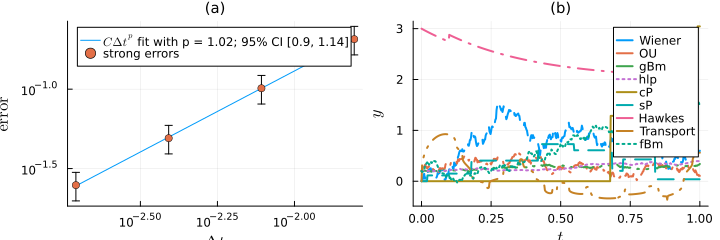
\includegraphics[scale=0.5]{img/allnoises_combined.png}
    \caption{(a) Order of convergence $p = 1.02$ of the strong error of the Euler method for $\mathrm{d}\mathbf{X}_t/\mathrm{d}t = - \left\|\mathbf{Y}_t\right\|^2 \mathbf{X}_t + \mathbf{Y}_t,$ on $[0, T] = [0.0, 1.0]$, with $\mathbf{X}_0 \sim \mathcal{N}(\mathbf{0}, \mathbf{I})$, and a vector-valued noise with different types of noise processes, computed with $M = 200$ sample paths, for each $\Delta t = 1/N$, with $N = 64,$ $128,$ $256,$ and $512.$; (b) Sample paths of all the noises used in the linear system \eqref{allnoisesRODEsystem}, mixing all different types of implemented noises.}
    \label{figallnoises}
\end{figure}

Table \ref{taballnoises} shows the estimated strong error obtained from 200 sample paths for each chosen time step, with initial condition $\mathbf{X}_0 \sim \mathcal{N}(\mathbf{0}, \mathrm{I})$, i.e. normally distributed on each coordinate, independently of the other coordinates, and on the time interval $[0.0, 1.0]$. \cref{figallnoises} illustrates the order of convergence and sample paths of all the noises used in this system.

The strong order 1 convergence is not a suprise in the case of the Wiener and Ornstein-Uhlenbeck process since the corresponding RODE can be turned into an SDE with an additive noise. In this case, the Euler-Maruyama approximation for the noise part of the SDE is distributionally exact, and the Euler method for the RODE becomes equivalent to the Euler-Maruyama method for the SDE. Moreover, it is known that the Euler-Maruyama method for an SDE with additive noise is of strong order 1 \cite{HighamKloeden2021}. For the remaining noises, however, previous works would estimate the order of convergence to be below the order 1 attained here. 

\subsection{Fractional Brownian motion noise}
\label{secfBmnoise}

Here, we consider again a linear equation, of the form
\begin{equation}
    \label{linearnonhomogeneousfbm}
    \begin{cases}
        \displaystyle \frac{\mathrm{d}X_t}{\mathrm{d} t} = -X_t + B^H_t, \qquad 0 \leq t \leq T, \\
        \left. X_t \right|_{t = 0} = X_0,
      \end{cases}
\end{equation}
except now the noise $\{B^H_t\}_t$ is assumed to be a fractional Brownian motion (fBm) with Hurst parameter $0 < H < 1$. It turns out that, for $0 < H < 1/2$, the order of convergence is $H + 1/2$. The same seems to hold for a nonlinear dependency on the fBm, but the proof is more involved, depending on a fractional It\^o formula (see \cite[Theorem 4.2.6]{BHOB2008}, \cite[Theorem 4.1]{Bender2003}and \cite[Theorem 2.7.4]{Mishura2008}), based on the Wick It\^o Skorohod (WIS) integral (see \cite[Chapter 4]{BHOB2008}). A corresponding WIS isometry is also needed (see e.g. \cite[Theorem 4.5.6]{BHOB2008}), involving Malliavin calculus and fractional derivatives. For these reasons, we leave the nonlinear case to a subsequent work and focus on this simple linear example, which suffices to illustrate the peculiarity of the dependence on $H$ of the order of convergence.

Although the above linear equation has the explicit solution
\begin{equation}
    X_t = e^{-t}X_0 + \int_0^t e^{-(t-s)}B^H_s\;\mathrm{d}s,
\end{equation}
computing a distributionally exact solution of this form is a delicate process. Thus we check the convergence numerically by solving the equation with the Euler method itself, but on a much finer mesh.

Indeed, we need to estimate the last term of \eqref{expectedestimateglobalerrorintegral}, in \eqref{propbasicestimate}, involving the steps of the term $f(t, x, y) = -x + y$, which in this case reduce to
\begin{equation}
    \label{stepfBm}
    f(s, X_{\tau^N(s)}^N, Y_s) - f(\tau^N(s), X_{\tau^N(s)}^N, Y_{\tau^N(s)}) = B^H_s - B^H_{\tau^N(s)},
\end{equation}
for $0 \leq s \leq T$. Using the representation \cite[eq. (2.1)]{MandelbrotVanNess1968}, \cite[eq. (1.1)]{BHOB2008} of an fBm, one can show after some calculations, that
\begin{multline}
    \mathbb{E}\left[\left|\int_0^{t_j} \left( f(s, X_{\tau^N(s)}^N, Y_s) - f(\tau^N(s), X_{\tau^N(s)}^N, Y_{\tau^N(s)}) \right)\;\mathrm{d}s\right|\right] \\
    \leq C_H^{(4)} \Delta t_N + C_H^{(3)} \Delta t_N^{H + 1/2},
\end{multline}
where $C_H^{(4)} = C_H^{(1)} + C_H^{(2)}$. Applying this estimate to \eqref{propbasicestimate} shows that the Euler method is of order $H + 1/2$, when $0 < H < 1/2$, and is of order 1, when $1/2 \leq H < 1$, having in mind that $H=1/2$ corresponds to the classical Wiener process.

As for the numerics, the Euler approximation is implemented for \eqref{linearnonhomogeneousfbm} with several values of $H$. We fix the time interval as $[0, T] = [0.0, 1.0]$, set the resolution for the target approximation to $N_{\textrm{tgt}} = 2^{19}$, choose the time steps for the convergence test as $\Delta t = 1/N$,  $N = 64,$ $128,$ $256,$ and $512,$ and use $M=200$ samples for the Monte-Carlo estimate of the strong error. The fBm noise term is generated with the $\mathcal{O}(N)$ fast Fourier transform (FFT) method of Davies and Harte, as presented in \cite{DiekerMandjes2003} (see also \cite[Section 14.4]{HanKloeden2017}). Table \ref{taborderdepHfBm} shows the obtained convergence estimates, for a series of Hurst parameters, which is illustrated in Figure \ref{figorderdepHfBm}.

\begin{table}
    \begin{tabular}[htb]{|c|c|}
        \hline H & p \\
        \hline \hline
        0.1 & 0.630713 \\
        0.2  & 0.759896 \\
        0.3  & 0.855504 \\
        0.4  & 0.942058 \\
        0.5  & 1.0012 \\
        0.7  & 1.00544 \\
        0.9  & 0.99782 \\
        \hline
    \end{tabular}
    \bigskip

    \caption{Hurst parameter $H$ and order $p$ of strong convergence for a number of Hurst values.}
    \label{taborderdepHfBm}
\end{table}

\begin{figure}[htb]
    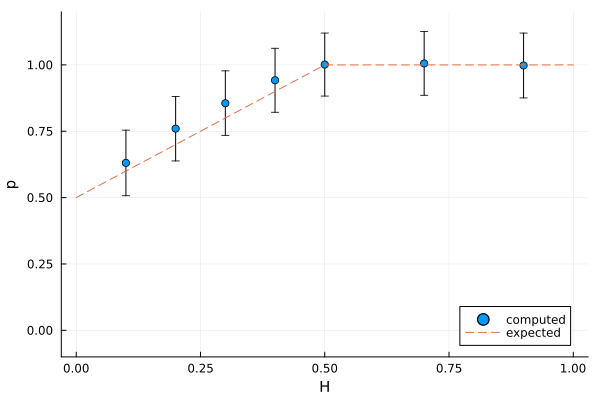
\includegraphics[scale=0.4]{img/order_dep_on_H_fBm.png}
    \caption{Order $p$ of strong convergence for each value of the Hurst parameter $H$ (scattered plot) along with the theoretical value $p=\min\{H + 1/2, 1\}$ (dashed line).}
    \label{figorderdepHfBm}
\end{figure}

\begin{thebibliography}{25}
    \bibitem{Asai2016} Y. Asai, \emph{Numerical Methods for Random Ordinary Differential Equations and their Appli-
    cations in Biology and Medicine.} Dissertation, Institut f\"ur Mathematik, Goethe Universit\"at Frankfurt am Main, 2016. 

    \bibitem{Bender2003} C. Bender, An It\^o formula for generalized functionals of a fractional Brownian motion with arbitrary Hurst parameter, \emph{Stochastic Processes and their Applications,} 104 (2003), 81--106.

    \bibitem{Julia2017} J. Bezanson, A. Edelman, S. Karpinski, and V. B. Shah, Julia: A fresh approach to numerical computing, \emph{Siam Review,} 59 (2017), no. 1, 65--98.

    \bibitem{BHOB2008} F. Biagini, Y. Hu, B. {\O}ksendal, and T. Zhang. \emph{Stochastic Calculus for Fractional Brownian Motion and Applications,} Springer-Verlag, London, 2008.

    \bibitem{BogdanoffGoldbergBernard1961} J. L. Bogdanoff, J. E. Goldberg, and M. C. Bernard, Response of a simple structure to a random earthquake-type disturbance, \emph{Bulletin of the Seismological Society of America,} 51 (1961), no. 2, 293--310.

    \bibitem{Clark1987} D. S. Clark, Short proof of a discrete Gronwall inequality, \emph{Discrete Applied Mathematics,} Vol. 16 (1987) no. 3, 279--281.

    \bibitem{CoddingtonLevinson1985} E. A. Coddington and N. Levinson, \emph{Theory of Ordinary Differential Equations,} New York: McGraw-Hill, 1987.

    \bibitem{DiekerMandjes2003} A. B. Dieker and M. Mandjes, On spectral simulation of fractional Brownian motion, \emph{Probability in the Engineering and Informational Sciences,} 17 (2003), 417--434.

    \bibitem{Fisher1937} R. A. Fisher, The wave of advance of advantageous genes, \emph{Annals of Eugenics,} 7 (1937), no. 4, 355--369.

    \bibitem{FreidlinWentzell1992} M. I. Freidlin and A. D. Wentzell, Reaction-diffusion equations with randomly perturbed boundary conditions, \emph{Ann. Probab.} 20 (1992), no. 2, 963--986.

    \bibitem{GHLOUZ1993} H. Gjessing, H. Holden, T. Lindstr{\o}n, B. {\O}ksendal, J. Ub{\o}e, and T.-S. Zhang, The Wick product, \emph{Vol. 1 Proceedings of the Third Finnish-Soviet Symposium on Probability Theory and Mathematical Statistics,} Turku, Finland, August 13--16, 1991, edited by H. Niemi, G. H\"ognas, A. N. Shiryaev and A. V. Melnikov, Berlin, Boston: De Gruyter, 1993, pp. 29-67.

    \bibitem{GiraultRaviart1981} V. Girault and P.-A. Raviart, \emph{Finite-Element Approximation of the Navier-Stokes Equations,} Lecture Notes in Mathematics, vol. 749, Springer-Verlag, Berlin, Heidelberg, 1981.

    \bibitem{Gronwall1919} T. H. Gronwall, Note on the derivatives with respect to a parameter of the solutions of a system of differential equations, \emph{Ann. of Math.} (2) 20 (1919), 292--296.

    \bibitem{GruneKloeden2001} L. Gr\"une and P.E. Kloeden, Higher order numerical schemes for affinely controlled nonlinear systems, \emph{Numer. Math.} 89 (2001), 669--690.

    \bibitem{HanKloeden2017} X. Han and P. E. Kloeden, \emph{Random Ordinary Differential Equations and Their Numerical Solution,} Probability Theory and Stochastic Modelling, vol. 85, Springer Singapore, 2017.

    \bibitem{HighamKloeden2021} D. J. Higham and P. E. Kloeden, \emph{An Introduction to the Numerical Simulation of Stochastic Differential Equations,} Volume 169 of Other Titles in Applied Mathematics, SIAM, 2021.

    \bibitem{HousnerJenning1964} G. W. Housner and Paul C. Jennings, Generation of artificial Earthquakes, Journal of the Engineering Mechanics Division, 90 (1964), no. 1.

    \bibitem{JentzenKloeden2011} A. Jentzen and P.E. Kloeden, \emph{Taylor Approximations of Stochastic Partial Differential Equations,} CBMS Lecture series, SIAM, Philadelphia, 2011.

    \bibitem{JentzenKloedenNeuenkirch2009} A. Jentzen, P.E. Kloeden, and A. Neuenkirch, Pathwise approximation of stochastic differential equations on domains: Higher order convergence rates without global Lipschitz coefficients, \emph{Numer. Math.} 112 (2009), no. 1, 41--64.

    \bibitem{Kanai1957} K. Kanai, Semi-empirical formula for the seismic characteristics of the ground, \emph{Bull. Earthq. Res. Inst.,} Vol. 35 (1957), University of Tokyo.

    \bibitem{KPP1937} A. N. Kolmogorov, I. G. Petrovskii, N. S. Piskunov, A study of the diffusion equation with increase in the amount of substance, and its application to a biological problem. \emph{Bull. Moscow Univ. Math. Mech.} 1 (1937), 1--26.

    \bibitem{Kuo2006} H.-H. Kuo, Introduction to Stochastic Integration, Springer, 2006.

    \bibitem{MandelbrotVanNess1968} B. B. Mandelbrot and J. W. Van Ness, Fractional Brownian Motions, Fractional Noises and Applications, \emph{Siam Review,} Vol. 10 (1968), no. 4, 422--437.

    \bibitem{Mishura2008} Y. S. Mishura, \emph{Stochastic calculus for fractional Brownian motion and related processes,} Lecture Notes in Mathematics 1929, Springer-Verlag, Berlin, Heidelberg, 2008.

    \bibitem{NeckelRupp2013} T. Neckel and F. Rupp, \emph{Random Differential Equations in Scientific Computing,} Versita, London, 2013.

    \bibitem{Oksendal2003} B. {\O}ksendal, \emph{Stochastic Differential Equations - An Introduction with Applications,} Universitext, Springer-Verlag Berlin Heidelberg, 2003.

    \bibitem{Protter2005} P. E. Protter, \emph{Stochastic Integration and Differential Equations,} 2nd Edition, Springer-Verlag, Berlin Heidelberg New York, 2005.

    \bibitem{RackauckasNie2017} C. Rackauckas and Q. Nie, DifferentialEquations.jl - A Performant and Feature-Rich Ecosystem for Solving Differential Equations in Julia, \emph{The Journal of Open Research Software}, 5 (2017), no. 1, 1--15.

    \bibitem{RODEConvEM2023} P. Kloeden and R. Rosa, Numerical examples of strong order of convergence of the Euler method for random ordinary differential equations, \texttt{https://github.com/rmsrosa/rode\_conv\_em}.

    \bibitem{SalakoShen2020} R. B. Salako and W. Shen, Long time behavior of random and nonautonomous Fisher-KPP equations: Part I - stability of equilibria and spreading speeds, \emph{J. Dyn. Diff. Eqs.,} 33 (2021), 1035--1070.

    \bibitem{StrasserTheisMarr2012} M. Strasser, F. J. Theis, and C. Marr, Stability and multiattractor dynamics of a toggle switch based on a two-stage model of stochastic gene expression, \emph{Biophysical J.,} 102 (2012), 19--29.

    \bibitem{Tajimi1960} H. Tajimi, A statistical method of determining the maximum response of a building during an Earthquake, \emph{Proceedings of the Second World Conference on Earthquake Engineering,} Tokyo and Kyoto, Japan, vol. II, 1960.
    
    \bibitem{VerdCrombachJaeger2014} B. Verd, A. Crombach, and J. Jaeger, Classification of transient behaviours in a time-dependent toggle switch model, \emph{BMC Systems Biology,} 8 (2014), no. 43.

    \bibitem{WangCaoHanKloeden2021} P. Wang, Y. Cao, X. Han, and P. Kloeden, Mean-square convergence of numerical methods for random ordinary differential equations, \emph{Numerical Algorithms,} vol. 87 (2021), 299--333.

\end{thebibliography}

\end{document}